% ---------------------------------------------------------------------
% Das Dokument kompiliert mit pdflatex und ist auf Basis
% von Koma-Script entstanden.
%
% Autor des Templates (für Anmerkungen):
% Michael von Riegen, riegen@informatik.uni-hamburg.de
%
% Einzelne Code-Teile für das Titelblatt sind aus dem Template
% von Benjamin Kirchheim entnommen.
%
% 25.05.09, Frank Langanke: Vorlage auf aktuelle KOMA-Version aktualisiert
% 26.05.09, Michael von Riegen: Anmerkung --> aktuelles Koma-Script ist nötig!
% 17.10.2016 neues Uni logo
% ---------------------------------------------------------------------
\documentclass[11pt,DIV=15,BCOR=20mm,bibliography=totoc]{scrbook}

% Import von Paketen und Optionen die das gesamte Dokument betreffen
% sind in myPreamble.sty ausgelagert.
\usepackage{myPreamble}

% Arbeitet man nur an einem Kapitel, wird durch folgenden Befehl nur dieses eingebunden.
% Spart manuelles auskommentieren von vielen include-Befehlen;
% hat keine Auswirkung auf input-Befehle
% \includeonly{kapitel1}

\begin{document}

% TITELSEITE
\begin{titlepage}

	% Fehler "destination with the same identifier" unterdrücken...
  \setcounter{page}{-1}

	% Titelseite
	\begin{figure}[h]
		\begin{minipage}[b]{62mm}
			
\includegraphics[width=62mm]{images/unilogo}
		\end{minipage}
		\hspace{4cm}
		\begin{minipage}[b]{59mm}
			
\includegraphics[width=59mm]{images/minlogo}
		\end{minipage}
	\end{figure}

	\vfill

	\begin{center}
		% Diplomarbeit
		\noindent { \Large
			Bachelor's Thesis \\
		}
		\vspace{14mm}
		% Titel
		\noindent \textbf{\huge
		A Recommender Framework for Skills Management \\
		%   Make Skills Management Great Again\\
		}
		\vspace{14mm}
    \noindent { \Large
			In Cooperation With SinnerSchrader \\
			% Design and Implementation of a Skills Management Web Application \\
		}
	\end{center}

	\vfill

	\noindent \textbf{Torben Reetz} \\
	\noindent \rule{\textwidth}{0.4mm}
	\noindent{\textrm{3reetz@informatik.uni-hamburg.de}} \\
	\noindent{\textrm{B.Sc. Software Systems Development}} \\
	\noindent{\textrm{Matr.-Nr. 6524064}} \\
	\noindent{\textrm{Semester 07}} \\
	\begin{tabbing}
	\hspace{8em} \=  \kill
	Primary Supervisor: Prof. Dr. Walid Maalej \\
	Secondary Supervisor: Prof. Dr. Eva Bittner \\
	~ \\
	Date: xx.xx.2017
	\end{tabbing}

	% Rückseite der Titelseite mit Zitat
	% \newpage
	% \thispagestyle{empty}
	% \setcounter{page}{0}

	% wenn man Lust auf ein Zitat hat...
	% ... ansonsten auskommentieren
	% ~\\ \vfill \noindent
	% A distributed system is one where the failure of some \\
	% computer I've never heard of can keep me from getting my work done. \\
	% \textit{-- Leslie Lamport}
\end{titlepage}


% VERZEICHNISSE (Inhaltsverzeichnis, Abkürzungen)
% Vorspann einleiten --> Seitennummerierung römisch
\frontmatter

\chapter{Abstract}
TODO alles muss neu, alles muss besser!
% Project driven organizations have to face the problem of constantly needing to put teams together based on the members’ skills, experience, motivation and preferences. At SinnerSchrader, like in many businesses, there is no central source of information about this data. Commercial solutions only take into account the employee’s knowledge whereas motivation and preferences will be ignored.
% This thesis covers the design and partial implementation of a web application that provides a search function to find the most suitable employee for a searched skill set based not only on their skills but also on their motivation.
% Usage scenarios and requirements that should be fulfilled by the system will be outlined. The design and realization of the application’s backend based on those requirements will be drafted and evaluated. To validate that the scoring algorithm created for this application is capable of fulfilling the users’ needs, a survey will be conducted and interpreted.


% Contentseses
\tableofcontents
% \cleardoublepage

% Hauptteil einleiten --> Seitennummerierung wieder arabisch
\mainmatter

%% -----------------------------------------------------------------------
% -----------------------------------------------------------------------
% -----------------------------------------------------------------------
% Einleitung
% -----------------------------------------------------------------------
% -----------------------------------------------------------------------
% -----------------------------------------------------------------------
\chapter{Einleitung}

Hier kommt eine Quellenangabe \cite{Gray1981}, \cite{Cerami2002}. Weiterhin sieht man hier einen Link auf Kapitel \ref{ch:1}. Lorem ipsum dolor sit amet, consectetuer\footnote{Hier ist eine Fußnote!} adipiscing elit. Integer quis lectus eget purus auctor sollicitudin. Sed tempus, leo quis nonummy iaculis, tellus justo bibendum mi, eu facilisis est sapien non eros. Ut tincidunt. Proin eleifend tristique est. Nulla facilisi. Cras ante mauris, facilisis at, fringilla quis, venenatis ornare, libero. Nam viverra varius nibh. Suspendisse potenti. Sed velit quam, euismod quis, sagittis eu, sodales sit amet, dui. Sed sed diam. Vivamus tincidunt quam a eros. Ut quis metus. Lorem ipsum dolor sit amet, consectetuer adipiscing elit. Cum sociis natoque penatibus et magnis dis parturient montes, nascetur ridiculus mus. Sed ut tortor. Vestibulum ante ipsum primis in faucibus orci luctus et ultrices posuere cubilia Curae; Curabitur vulputate nibh a tortor. Nullam scelerisque risus nonummy urna tempor sagittis.

\noindent Hier kommt ein Listing \ref{lst:soap}.

\begin{center}
\begin{lstlisting}[caption={SOAP Anfrage an einen HalloWelt-Web-Service},label=lst:soap,language=XML,label={lst:soap}]
<?xml version='1.0' encoding='UTF-8'>
<SOAP-ENV:Envelope (*@\label{lst:soapEnv}@*)
  xmlns:SOAP-ENV="http://schemas.xmlsoap.org/soap/envelope/"
  xmlns:xsi="http://www.w3.org/2001/XMLSchema-instance"
  xmlns:xsd="http://www.w3.org/2001/XMLSchema"
  xmlns:ns1="http://localhost/wsdl/HalloWeltService.wsdl">
  
  <SOAP-ENV:Body>(*@\label{lst:soapBody}@*)
  	<ns1:gruss>
  		<name xsi:type="xsd:string">
  			Michael
  		</name>
  	</ns1:gruss>
  </SOAP-ENV:Body>

</SOAP-ENV:Envelope>
\end{lstlisting}
\end{center}

Donec tincidunt. Cras tempus purus et quam. Duis semper. Vestibulum eu ligula. Ut non odio. Ut posuere ligula fringilla neque. Cras sodales justo eu massa. Nullam mauris nulla, fermentum et, fringilla sed, imperdiet vitae, turpis. In vehicula fermentum neque. Cum sociis natoque penatibus et magnis dis parturient montes, nascetur ridiculus mus. Quisque orci. Nunc odio. Nam consectetuer egestas augue.

\noindent Hier kommt eine etwas komplizierte Tabelle:

\begin{table}[h]
	\caption[Transaktionale Ablaufmodelle im Vergleich]{Transaktionale Ablaufmodelle im Vergleich; teilweise aus \cite{DBLP:books/infix/Schwarz99}; das Wort "`Transaktion"' wird in der Tabelle als TA abgekürzt}
	\label{tab:tamodelleVergleich}
	\centering
		\begin{tabular*}{\textwidth}{| l@{\extracolsep\fill} r || c | c | c || c | c || c || c || c | c | c || c | c |}
			\hline
			
			Modelle & 
				\rotatebox{90}{Eigenschaften} &
					\rotatebox{90}{vital} &
						\rotatebox{90}{non-vital} &
							\rotatebox{90}{Alternativtransaktion } &				
								\rotatebox{90}{sequenziell} &
									\rotatebox{90}{parallel} &
  									\rotatebox{90}{unabhängig} &
	    								\rotatebox{90}{temporal} &
			    							\rotatebox{90}{geschlossen geschachtelt } &
					    						\rotatebox{90}{offen geschachtelt} &
							    					\rotatebox{90}{Kompensation} &
									    				\rotatebox{90}{endliche Schachtelung } &
											    			\rotatebox{90}{unendliche Schachtelung } \\
			
			\hline
			\hline
			
			\multicolumn{2}{|l||}{Geschl. gesch. TA} &
				\checkmark &
				 (\checkmark) &
				 	(\checkmark) &
				 		\checkmark &
				 			\checkmark &
				 			
				 			  - &
				 			  - &
				 			
				 				\checkmark &
				 				  - &
				 				  	-	&
				 				  		\checkmark &
				 				  			\checkmark \\
			\hline

			\multicolumn{2}{|l||}{Offen gesch. TA} &
				\checkmark &
				 (\checkmark) &
				 	(\checkmark) &
				 		\checkmark &
				 			\checkmark &
				 			 
				 			  - &
				 			  - &
				 			
				 				- &
				 				  \checkmark &
				 				  	\checkmark &
				 				  		\checkmark &
				 				  			\checkmark \\
			\hline

			\multicolumn{2}{|l||}{Sagas} &
				\checkmark &
				 - &
				 	- &
				 		\checkmark &
				 			- &
				 			
				 			  - &
				 			  - &
				 			
				 				- &
				 				  \checkmark &
				 				  	\checkmark &	
				 				  		\checkmark &
				 				  			- \\
			\hline

			\multicolumn{2}{|l||}{Flex-TA} &
				\checkmark &
				 \checkmark &
				 	\checkmark &
				 		\checkmark &
				 			\checkmark &
				 			
				 			- &
				 			\checkmark &
				 			 
				 			
				 				\checkmark &
				 				  \checkmark &
				 				  	\checkmark &
				 				  		\checkmark &
				 				  			- \\
			
			\hline

			\multicolumn{2}{|l||}{ConTracts} &
				\checkmark &
				 \checkmark &
				 	- &
				 		\checkmark &
				 			\checkmark &
				 			
				 			 -&
				 			 -&
				 			
				 				\checkmark &
				 				  \checkmark &
				 				  	\checkmark &
				 				  		\checkmark &
				 				  			\checkmark \\

			\hline

			\multicolumn{2}{|l||}{Business-TA} &
				\checkmark &
				 \checkmark &
				 	\checkmark &
				 		\checkmark &
				 			\checkmark &

  			 			 \checkmark &
				 			 \checkmark &
				 			  
				 				\checkmark &
				 				  \checkmark &
				 				  	\checkmark &
				 				  		\checkmark &
				 				  			\checkmark \\			 				  			
			\hline
				
		\end{tabular*}
\end{table}

Vestibulum sed odio. Mauris semper placerat ipsum. Nulla facilisi. In rutrum, tortor in rhoncus venenatis, diam enim lacinia urna, vel egestas nunc sapien ut nisl. Fusce placerat posuere est. Maecenas augue. In gravida leo vel massa. Aliquam eu nisi. Cras tincidunt aliquam arcu. Pellentesque habitant morbi tristique senectus et netus et malesuada fames ac turpis egestas. Aenean quis libero condimentum libero porttitor vestibulum. Pellentesque a nulla nec ipsum tristique molestie.

Curabitur sagittis quam vitae tortor. Nulla id pede. Praesent rutrum, ipsum quis porttitor pretium, nisl ipsum gravida est, commodo pulvinar augue nibh ac felis. Aliquam erat volutpat. Aenean ullamcorper feugiat dolor. Donec nulla mauris, elementum sed, varius ut, blandit vitae, purus. Aenean in nunc in justo sodales fringilla. Proin pulvinar. Maecenas ullamcorper. Vivamus dapibus consectetuer arcu. Nam dictum, erat non adipiscing pretium, lorem tellus pulvinar dui, ut condimentum massa est sit amet urna. Nulla facilisi.

Vivamus in dui. Morbi tristique nibh in purus. Nam erat. Curabitur euismod lacinia purus. Maecenas tempor libero quis dolor. Quisque gravida lorem vitae libero. Aliquam sodales, risus in tempor imperdiet, massa nisi auctor massa, vitae laoreet nunc erat in sapien. Etiam eu sapien nec enim consectetuer accumsan. Nunc non quam. Cras placerat justo quis nibh nonummy sollicitudin. Aenean vitae felis. Mauris id mi nec ligula ultricies vestibulum. Suspendisse luctus pretium justo. 

\section{Motivation}
\label{ch:1}
Lorem ipsum dolor sit amet, consectetuer adipiscing elit. Integer quis lectus eget purus auctor sollicitudin. Sed tempus, leo quis nonummy iaculis, tellus justo bibendum mi, eu facilisis est sapien non eros. Ut tincidunt. Proin eleifend tristique est. Nulla facilisi. Cras ante mauris, facilisis at, fringilla quis, venenatis ornare, libero. Nam viverra varius nibh. Suspendisse potenti. Sed velit quam, euismod quis, sagittis eu, sodales sit amet, dui. Sed sed diam. Vivamus tincidunt quam a eros. Ut quis metus. Lorem ipsum dolor sit amet, consectetuer adipiscing elit. Cum sociis natoque penatibus et magnis dis parturient montes, nascetur ridiculus mus. Sed ut tortor. Vestibulum ante ipsum primis in faucibus orci luctus et ultrices posuere cubilia Curae; Curabitur vulputate nibh a tortor. Nullam scelerisque risus nonummy urna tempor sagittis.

Donec tincidunt. Cras tempus purus et quam. Duis semper. Vestibulum eu ligula. Ut non odio. Ut posuere ligula fringilla neque. Cras sodales justo eu massa. Nullam mauris nulla, fermentum et, fringilla sed, imperdiet vitae, turpis. In vehicula fermentum neque. Cum sociis natoque penatibus et magnis dis parturient montes, nascetur ridiculus mus. Quisque orci. Nunc odio. Nam consectetuer egestas augue.

Vestibulum sed odio. Mauris semper placerat ipsum. Nulla facilisi. In rutrum, tortor in rhoncus venenatis, diam enim lacinia urna, vel egestas nunc sapien ut nisl. Fusce placerat posuere est. Maecenas augue. In gravida leo vel massa. Aliquam eu nisi. Cras tincidunt aliquam arcu. Pellentesque habitant morbi tristique senectus et netus et malesuada fames ac turpis egestas. Aenean quis libero condimentum libero porttitor vestibulum. Pellentesque a nulla nec ipsum tristique molestie.

Curabitur sagittis quam vitae tortor. Nulla id pede. Praesent rutrum, ipsum quis porttitor pretium, nisl ipsum gravida est, commodo pulvinar augue nibh ac felis. Aliquam erat volutpat. Aenean ullamcorper feugiat dolor. Donec nulla mauris, elementum sed, varius ut, blandit vitae, purus. Aenean in nunc in justo sodales fringilla. Proin pulvinar. Maecenas ullamcorper. Vivamus dapibus consectetuer arcu. Nam dictum, erat non adipiscing pretium, lorem tellus pulvinar dui, ut condimentum massa est sit amet urna. Nulla facilisi.

Vivamus in dui. Morbi tristique nibh in purus. Nam erat. Curabitur euismod lacinia purus. Maecenas tempor libero quis dolor. Quisque gravida lorem vitae libero. Aliquam sodales, risus in tempor imperdiet, massa nisi auctor massa, vitae laoreet nunc erat in sapien. Etiam eu sapien nec enim consectetuer accumsan. Nunc non quam. Cras placerat justo quis nibh nonummy sollicitudin. Aenean vitae felis. Mauris id mi nec ligula ultricies vestibulum. Suspendisse luctus pretium justo. 

Vestibulum sed odio. Mauris semper placerat ipsum. Nulla facilisi. In rutrum, tortor in rhoncus venenatis, diam enim lacinia urna, vel egestas nunc sapien ut nisl. Fusce placerat posuere est. Maecenas augue. In gravida leo vel massa. Aliquam eu nisi. Cras tincidunt aliquam arcu. Pellentesque habitant morbi tristique senectus et netus et malesuada fames ac turpis egestas. Aenean quis libero condimentum libero porttitor vestibulum. Pellentesque a nulla nec ipsum tristique molestie.

Curabitur sagittis quam vitae tortor. Nulla id pede. Praesent rutrum, ipsum quis porttitor pretium, nisl ipsum gravida est, commodo pulvinar augue nibh ac felis. Aliquam erat volutpat. Aenean ullamcorper feugiat dolor. Donec nulla mauris, elementum sed, varius ut, blandit vitae, purus. Aenean in nunc in justo sodales fringilla. Proin pulvinar. Maecenas ullamcorper. Vivamus dapibus consectetuer arcu. Nam dictum, erat non adipiscing pretium, lorem tellus pulvinar dui, ut condimentum massa est sit amet urna. Nulla facilisi.

Vivamus in dui. Morbi tristique nibh in purus. Nam erat. Curabitur euismod lacinia purus. Maecenas tempor libero quis dolor. Quisque gravida lorem vitae libero. Aliquam sodales, risus in tempor imperdiet, massa nisi auctor massa, vitae laoreet nunc erat in sapien. Etiam eu sapien nec enim consectetuer accumsan. Nunc non quam. Cras placerat justo quis nibh nonummy sollicitudin. Aenean vitae felis. Mauris id mi nec ligula ultricies vestibulum. Suspendisse luctus pretium justo. 

Vestibulum sed odio. Mauris semper placerat ipsum. Nulla facilisi. In rutrum, tortor in rhoncus venenatis, diam enim lacinia urna, vel egestas nunc sapien ut nisl. Fusce placerat posuere est. Maecenas augue. In gravida leo vel massa. Aliquam eu nisi. Cras tincidunt aliquam arcu. Pellentesque habitant morbi tristique senectus et netus et malesuada fames ac turpis egestas. Aenean quis libero condimentum libero porttitor vestibulum. Pellentesque a nulla nec ipsum tristique molestie.

Curabitur sagittis quam vitae tortor. Nulla id pede. Praesent rutrum, ipsum quis porttitor pretium, nisl ipsum gravida est, commodo pulvinar augue nibh ac felis. Aliquam erat volutpat. Aenean ullamcorper feugiat dolor. Donec nulla mauris, elementum sed, varius ut, blandit vitae, purus. Aenean in nunc in justo sodales fringilla. Proin pulvinar. Maecenas ullamcorper. Vivamus dapibus consectetuer arcu. Nam dictum, erat non adipiscing pretium, lorem tellus pulvinar dui, ut condimentum massa est sit amet urna. Nulla facilisi.

Vivamus in dui. Morbi tristique nibh in purus. Nam erat. Curabitur euismod lacinia purus. Maecenas tempor libero quis dolor. Quisque gravida lorem vitae libero. Aliquam sodales, risus in tempor imperdiet, massa nisi auctor massa, vitae laoreet nunc erat in sapien. Etiam eu sapien nec enim consectetuer accumsan. Nunc non quam. Cras placerat justo quis nibh nonummy sollicitudin. Aenean vitae felis. Mauris id mi nec ligula ultricies vestibulum. Suspendisse luctus pretium justo. 

Vestibulum sed odio. Mauris semper placerat ipsum. Nulla facilisi. In rutrum, tortor in rhoncus venenatis, diam enim lacinia urna, vel egestas nunc sapien ut nisl. Fusce placerat posuere est. Maecenas augue. In gravida leo vel massa. Aliquam eu nisi. Cras tincidunt aliquam arcu. Pellentesque habitant morbi tristique senectus et netus et malesuada fames ac turpis egestas. Aenean quis libero condimentum libero porttitor vestibulum. Pellentesque a nulla nec ipsum tristique molestie.

Curabitur sagittis quam vitae tortor. Nulla id pede. Praesent rutrum, ipsum quis porttitor pretium, nisl ipsum gravida est, commodo pulvinar augue nibh ac felis. Aliquam erat volutpat. Aenean ullamcorper feugiat dolor. Donec nulla mauris, elementum sed, varius ut, blandit vitae, purus. Aenean in nunc in justo sodales fringilla. Proin pulvinar. Maecenas ullamcorper. Vivamus dapibus consectetuer arcu. Nam dictum, erat non adipiscing pretium, lorem tellus pulvinar dui, ut condimentum massa est sit amet urna. Nulla facilisi.

Vivamus in dui. Morbi tristique nibh in purus. Nam erat. Curabitur euismod lacinia purus. Maecenas tempor libero quis dolor. Quisque gravida lorem vitae libero. Aliquam sodales, risus in tempor imperdiet, massa nisi auctor massa, vitae laoreet nunc erat in sapien. Etiam eu sapien nec enim consectetuer accumsan. Nunc non quam. Cras placerat justo quis nibh nonummy sollicitudin. Aenean vitae felis. Mauris id mi nec ligula ultricies vestibulum. Suspendisse luctus pretium justo. 

\section{Zielsetzung}
Lorem ipsum dolor sit amet, consectetuer adipiscing elit. Integer quis lectus eget purus auctor sollicitudin. Sed tempus, leo quis nonummy iaculis, tellus justo bibendum mi, eu facilisis est sapien non eros. Ut tincidunt. Proin eleifend tristique est. Nulla facilisi. Cras ante mauris, facilisis at, fringilla quis, venenatis ornare, libero. Nam viverra varius nibh. Suspendisse potenti. Sed velit quam, euismod quis, sagittis eu, sodales sit amet, dui. Sed sed diam. Vivamus tincidunt quam a eros. Ut quis metus. Lorem ipsum dolor sit amet, consectetuer adipiscing elit. Cum sociis natoque penatibus et magnis dis parturient montes, nascetur ridiculus mus. Sed ut tortor. Vestibulum ante ipsum primis in faucibus orci luctus et ultrices posuere cubilia Curae; Curabitur vulputate nibh a tortor. Nullam scelerisque risus nonummy urna tempor sagittis.

Donec tincidunt. Cras tempus purus et quam. Duis semper. Vestibulum eu ligula. Ut non odio. Ut posuere ligula fringilla neque. Cras sodales justo eu massa. Nullam mauris nulla, fermentum et, fringilla sed, imperdiet vitae, turpis. In vehicula fermentum neque. Cum sociis natoque penatibus et magnis dis parturient montes, nascetur ridiculus mus. Quisque orci. Nunc odio. Nam consectetuer egestas augue.

Vestibulum sed odio. Mauris semper placerat ipsum. Nulla facilisi. In rutrum, tortor in rhoncus venenatis, diam enim lacinia urna, vel egestas nunc sapien ut nisl. Fusce placerat posuere est. Maecenas augue. In gravida leo vel massa. Aliquam eu nisi. Cras tincidunt aliquam arcu. Pellentesque habitant morbi tristique senectus et netus et malesuada fames ac turpis egestas. Aenean quis libero condimentum libero porttitor vestibulum. Pellentesque a nulla nec ipsum tristique molestie.

Curabitur sagittis quam vitae tortor. Nulla id pede. Praesent rutrum, ipsum quis porttitor pretium, nisl ipsum gravida est, commodo pulvinar augue nibh ac felis. Aliquam erat volutpat. Aenean ullamcorper feugiat dolor. Donec nulla mauris, elementum sed, varius ut, blandit vitae, purus. Aenean in nunc in justo sodales fringilla. Proin pulvinar. Maecenas ullamcorper. Vivamus dapibus consectetuer arcu. Nam dictum, erat non adipiscing pretium, lorem tellus pulvinar dui, ut condimentum massa est sit amet urna. Nulla facilisi.

Vivamus in dui. Morbi tristique nibh in purus. Nam erat. Curabitur euismod lacinia purus. Maecenas tempor libero quis dolor. Quisque gravida lorem vitae libero. Aliquam sodales, risus in tempor imperdiet, massa nisi auctor massa, vitae laoreet nunc erat in sapien. Etiam eu sapien nec enim consectetuer accumsan. Nunc non quam. Cras placerat justo quis nibh nonummy sollicitudin. Aenean vitae felis. Mauris id mi nec ligula ultricies vestibulum. Suspendisse luctus pretium justo. 

\section{Eingrenzung des Themas}
\label{ch:eingrenzungThema}
Lorem ipsum dolor sit amet, consectetuer adipiscing elit. Integer quis lectus eget purus auctor sollicitudin. Sed tempus, leo quis nonummy iaculis, tellus justo bibendum mi, eu facilisis est sapien non eros. Ut tincidunt. Proin eleifend tristique est. Nulla facilisi. Cras ante mauris, facilisis at, fringilla quis, venenatis ornare, libero. Nam viverra varius nibh. Suspendisse potenti. Sed velit quam, euismod quis, sagittis eu, sodales sit amet, dui. Sed sed diam. Vivamus tincidunt quam a eros. Ut quis metus. Lorem ipsum dolor sit amet, consectetuer adipiscing elit. Cum sociis natoque penatibus et magnis dis parturient montes, nascetur ridiculus mus. Sed ut tortor. Vestibulum ante ipsum primis in faucibus orci luctus et ultrices posuere cubilia Curae; Curabitur vulputate nibh a tortor. Nullam scelerisque risus nonummy urna tempor sagittis.

Donec tincidunt. Cras tempus purus et quam. Duis semper. Vestibulum eu ligula. Ut non odio. Ut posuere ligula fringilla neque. Cras sodales justo eu massa. Nullam mauris nulla, fermentum et, fringilla sed, imperdiet vitae, turpis. In vehicula fermentum neque. Cum sociis natoque penatibus et magnis dis parturient montes, nascetur ridiculus mus. Quisque orci. Nunc odio. Nam consectetuer egestas augue.

Vestibulum sed odio. Mauris semper placerat ipsum. Nulla facilisi. In rutrum, tortor in rhoncus venenatis, diam enim lacinia urna, vel egestas nunc sapien ut nisl. Fusce placerat posuere est. Maecenas augue. In gravida leo vel massa. Aliquam eu nisi. Cras tincidunt aliquam arcu. Pellentesque habitant morbi tristique senectus et netus et malesuada fames ac turpis egestas. Aenean quis libero condimentum libero porttitor vestibulum. Pellentesque a nulla nec ipsum tristique molestie.

Curabitur sagittis quam vitae tortor. Nulla id pede. Praesent rutrum, ipsum quis porttitor pretium, nisl ipsum gravida est, commodo pulvinar augue nibh ac felis. Aliquam erat volutpat. Aenean ullamcorper feugiat dolor. Donec nulla mauris, elementum sed, varius ut, blandit vitae, purus. Aenean in nunc in justo sodales fringilla. Proin pulvinar. Maecenas ullamcorper. Vivamus dapibus consectetuer arcu. Nam dictum, erat non adipiscing pretium, lorem tellus pulvinar dui, ut condimentum massa est sit amet urna. Nulla facilisi.

Vivamus in dui. Morbi tristique nibh in purus. Nam erat. Curabitur euismod lacinia purus. Maecenas tempor libero quis dolor. Quisque gravida lorem vitae libero. Aliquam sodales, risus in tempor imperdiet, massa nisi auctor massa, vitae laoreet nunc erat in sapien. Etiam eu sapien nec enim consectetuer accumsan. Nunc non quam. Cras placerat justo quis nibh nonummy sollicitudin. Aenean vitae felis. Mauris id mi nec ligula ultricies vestibulum. Suspendisse luctus pretium justo. 

\section{Aufbau der Arbeit} 
Lorem ipsum dolor sit amet, consectetuer adipiscing elit. Integer quis lectus eget purus auctor sollicitudin. Sed tempus, leo quis nonummy iaculis, tellus justo bibendum mi, eu facilisis est sapien non eros. Ut tincidunt. Proin eleifend tristique est. Nulla facilisi. Cras ante mauris, facilisis at, fringilla quis, venenatis ornare, libero. Nam viverra varius nibh. Suspendisse potenti. Sed velit quam, euismod quis, sagittis eu, sodales sit amet, dui. Sed sed diam. Vivamus tincidunt quam a eros. Ut quis metus. Lorem ipsum dolor sit amet, consectetuer adipiscing elit. Cum sociis natoque penatibus et magnis dis parturient montes, nascetur ridiculus mus. Sed ut tortor. Vestibulum ante ipsum primis in faucibus orci luctus et ultrices posuere cubilia Curae; Curabitur vulputate nibh a tortor. Nullam scelerisque risus nonummy urna tempor sagittis.

Donec tincidunt. Cras tempus purus et quam. Duis semper. Vestibulum eu ligula. Ut non odio. Ut posuere ligula fringilla neque. Cras sodales justo eu massa. Nullam mauris nulla, fermentum et, fringilla sed, imperdiet vitae, turpis. In vehicula fermentum neque. Cum sociis natoque penatibus et magnis dis parturient montes, nascetur ridiculus mus. Quisque orci. Nunc odio. Nam consectetuer egestas augue.

Vestibulum sed odio. Mauris semper placerat ipsum. Nulla facilisi. In rutrum, tortor in rhoncus venenatis, diam enim lacinia urna, vel egestas nunc sapien ut nisl. Fusce placerat posuere est. Maecenas augue. In gravida leo vel massa. Aliquam eu nisi. Cras tincidunt aliquam arcu. Pellentesque habitant morbi tristique senectus et netus et malesuada fames ac turpis egestas. Aenean quis libero condimentum libero porttitor vestibulum. Pellentesque a nulla nec ipsum tristique molestie.

Curabitur sagittis quam vitae tortor. Nulla id pede. Praesent rutrum, ipsum quis porttitor pretium, nisl ipsum gravida est, commodo pulvinar augue nibh ac felis. Aliquam erat volutpat. Aenean ullamcorper feugiat dolor. Donec nulla mauris, elementum sed, varius ut, blandit vitae, purus. Aenean in nunc in justo sodales fringilla. Proin pulvinar. Maecenas ullamcorper. Vivamus dapibus consectetuer arcu. Nam dictum, erat non adipiscing pretium, lorem tellus pulvinar dui, ut condimentum massa est sit amet urna. Nulla facilisi.

Vivamus in dui. Morbi tristique nibh in purus. Nam erat. Curabitur euismod lacinia purus. Maecenas tempor libero quis dolor. Quisque gravida lorem vitae libero. Aliquam sodales, risus in tempor imperdiet, massa nisi auctor massa, vitae laoreet nunc erat in sapien. Etiam eu sapien nec enim consectetuer accumsan. Nunc non quam. Cras placerat justo quis nibh nonummy sollicitudin. Aenean vitae felis. Mauris id mi nec ligula ultricies vestibulum. Suspendisse luctus pretium justo. 

\chapter{SinnerSchrader}

The SinnerSchrader Group is a full service web agency based in Hamburg aggregating the subcompanies SinnerSchrader Deutschland, SinnerSchrader Content, SinnerSchrader Commerce and SinnerSchrader Swipe. The broad spectrum of expertise,including, but not limited to, digital communication strategies, visual and interaction design,  technical architecture, full stack development, editorial services, content production, E-Commerce, mobile app development, hosting, and maintenance, allows SinnerSchrader to serve all needs regarding their customer’s digital transformation. The combination of all said competencies under one single roof reduces organisational friction between the discipline-specific teams because they all share the same vision of the big picture they are creating. This does not only lead to faster development cycles, but also to a more coherent and unified product.

\subsection{Project-Driven Business}
As a web agency, it is clear that SinnerSchrader has to operate in a project-driven way. This means there no continuous stream of recurring work repeating constantly, but many different projects for different clients, each one dealing with varying challenges and questions. From a technical point of view, the diversity of know-how needed for each project is extremely huge since every application uses its own dedicated stack of technologies. As a consequence, the developers’ skill sets are based on the combination of projects they have worked on and their general field of interest. This results in one problem: Managers frequently have to put teams together based on the members’ skills with respect to the individual requirements of the project.\newline
This thesis will cover the creation of a tool helping managers with that problem by providing a centralized source of data about each employee’s professional abilities.
\newpage
\subsection{Matrix Organisation}
The personnel of SinnerSchrader are divided into two different kinds of teams: functional teams of
employees sharing the same specialization, i.E. backend development, frontend development, design, or concept, and project teams of people from different functional teams working collaboratively on the same project. This structural model is called a matrix organisation. \cite[P. 75]{BWL}
The organisational head of functional teams will further be called the `supervisor'; the pendant for project team will be mentioned as `team manager'.

\begin{figure}[!htp]
    \centering
    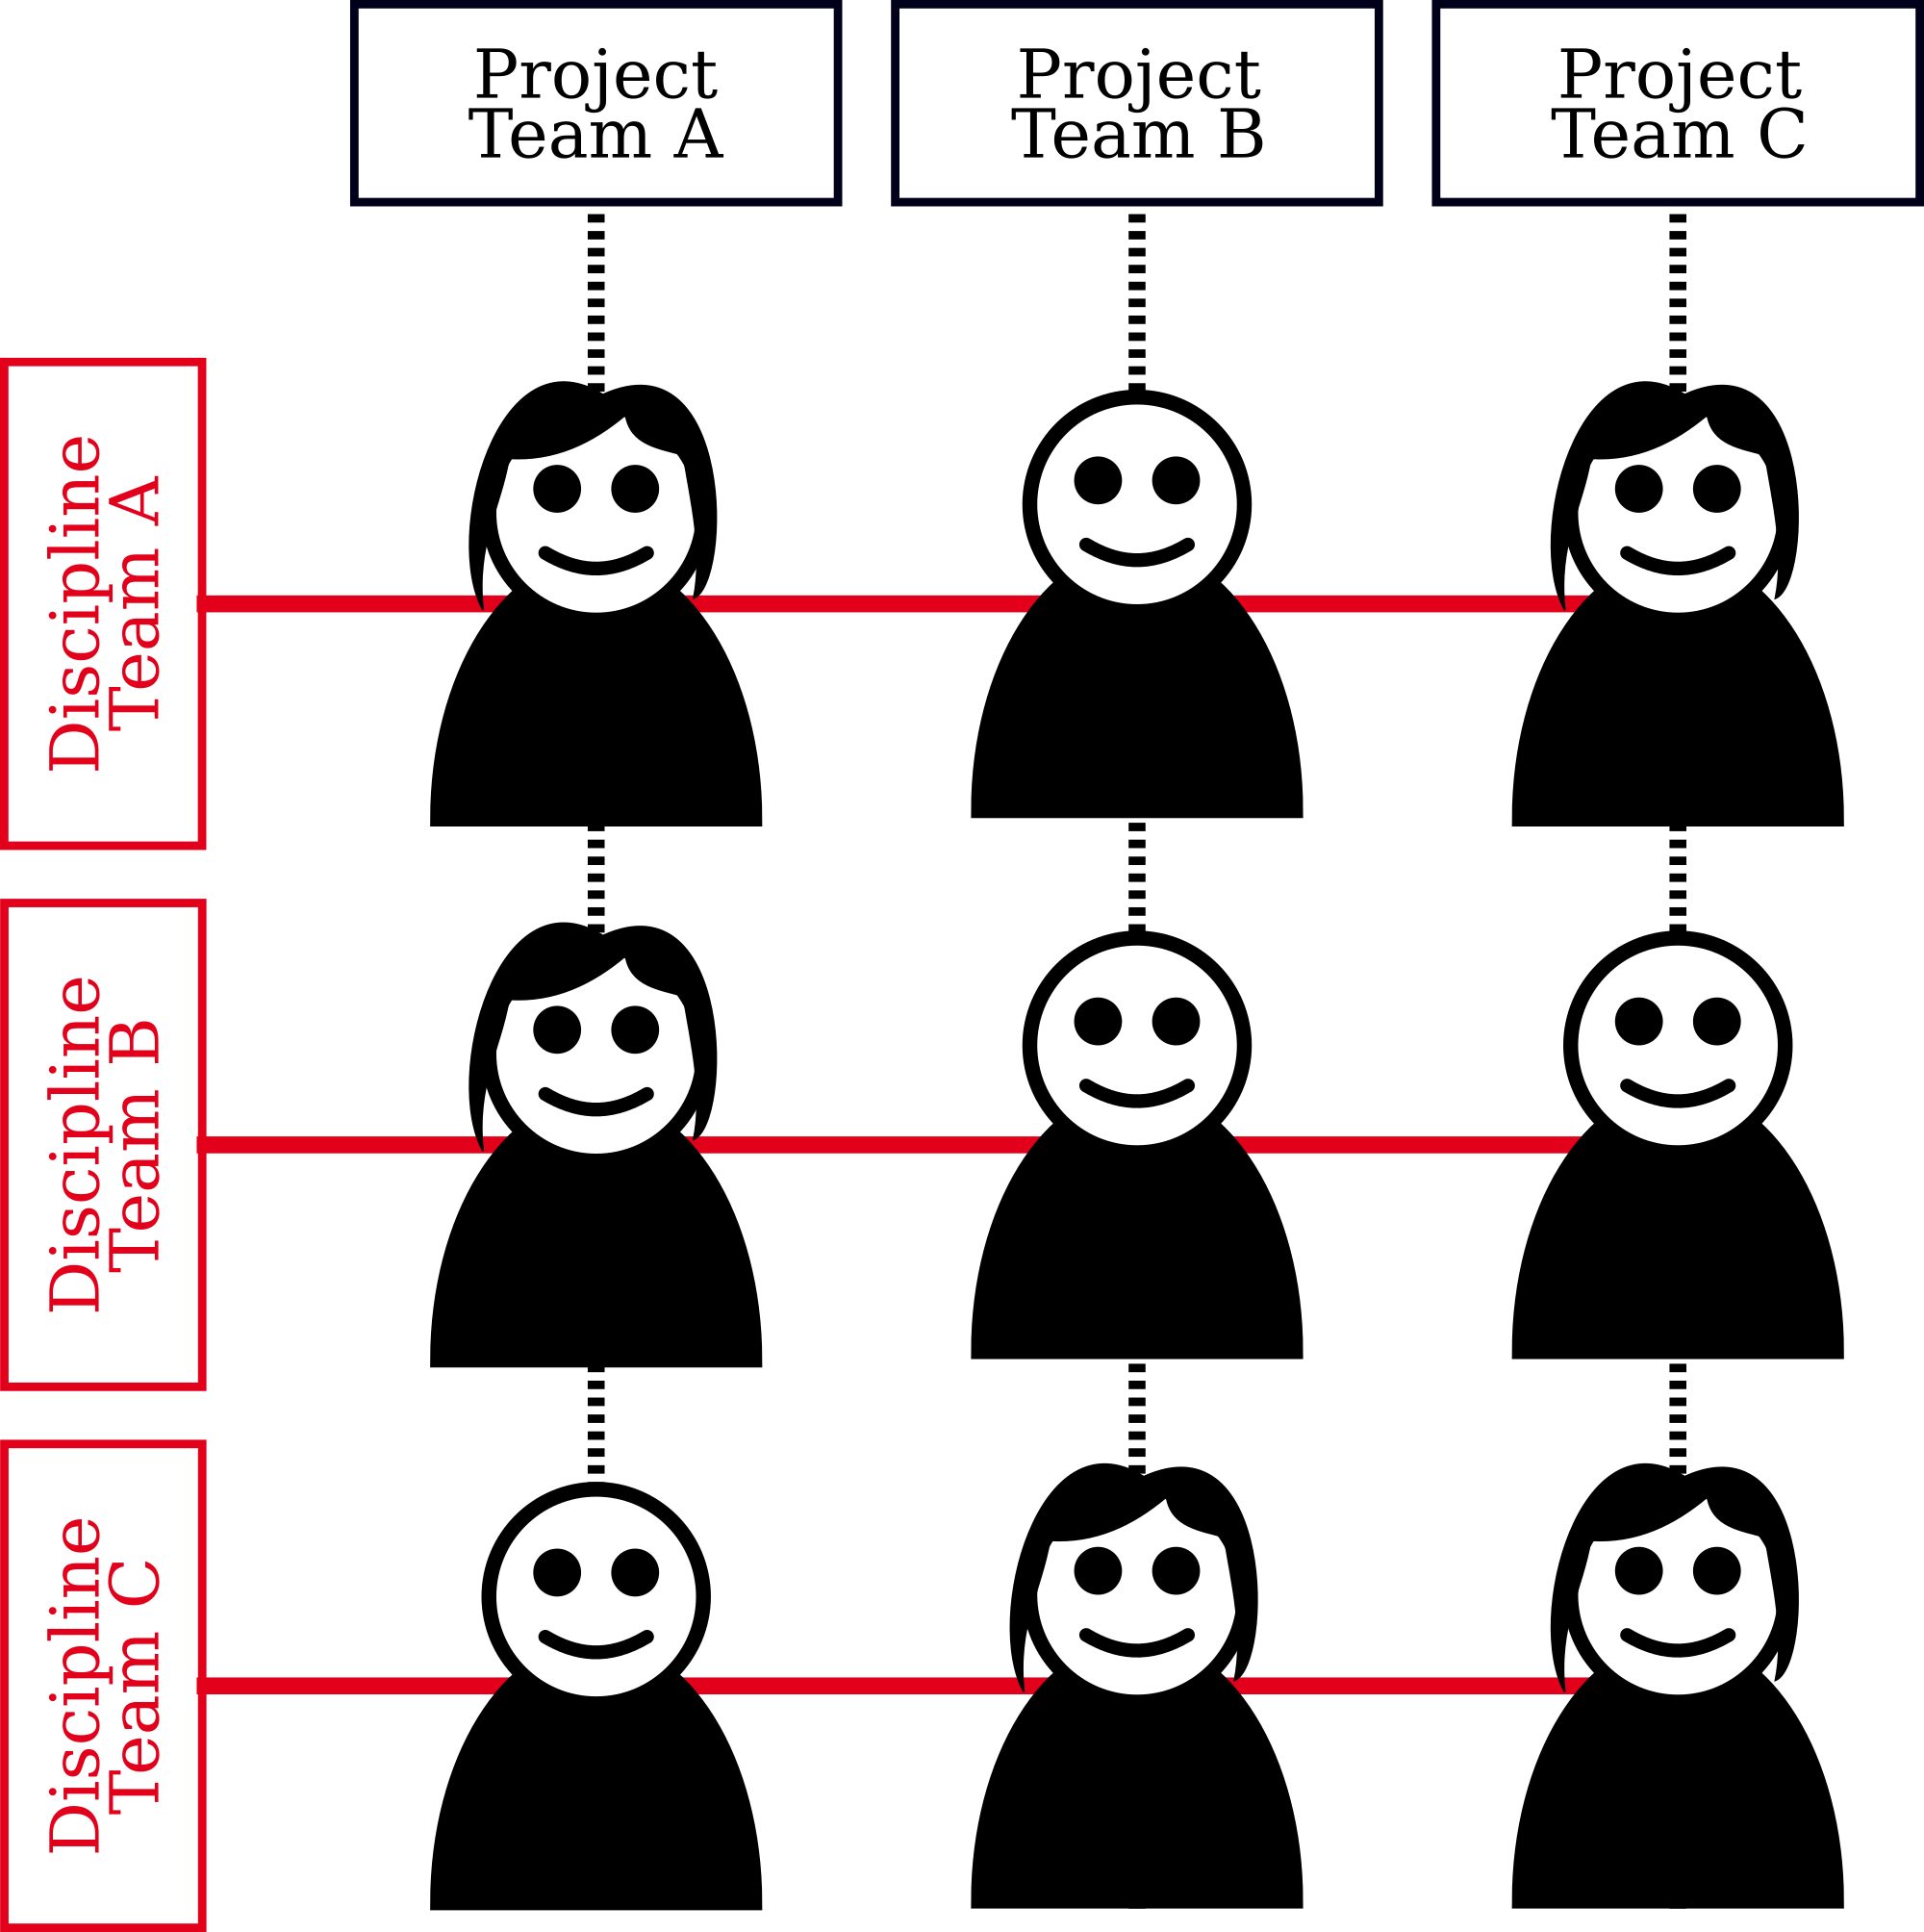
\includegraphics[width=0.33\textwidth]{images/matrixorga.png}
    \caption[Matrix Organisation]{Illustration of a matrix organisation}
    \label{fig:matrixorga}
\end{figure}

\chapter{Concept}
The application should be accessible to all employees of SinnerSchrader. Due to the heterogeneity of the the users' computer setups running \textit{Windows}, \textit{macOS} and \textit{Linux}, creating a native application supported by everyone’s system is a rather complicated task. A web application using standard technologies does not only solve this problem, but can also be used from mobile devices such as smartphones and tablets. Furthermore, there is no need to manually install and update the software so that it can be assumed that all users use the latest version of the application. This is a positive factor regarding the overall usability of the system and assures bugs and security issues are eliminated the moment a new version of the software is deployed. All those advantages compared to native clients and the fact that SinnerSchrader’s expertise lies in the development of web applications lead to the decision, that such an application would be the appropriate choice.

\section{Person Search}
The central feature of the application is the search function that returns a list of all persons matching the entered set of skills. By default, the results are ordered by a fitness score which describes how well a person matches into the set of searched skills. As a consequence of this sorting, the application implicitly recommends the best matching person to the user, thus it falls within the group of \textit{recommender systems}.

\subsection{Recommender Systems}
Recommender systems ``are information filtering systems that deal with the problem of information overload by filtering vital information fragment out of large amount of [...] information'' \cite{Isinkaye2015261}\label{recommender-definition} and are commonly used to recommend an item to the user based on their previous interactions with other items. For example, recommender systems are used to predict products a customer might want to buy based on the ones they already bought in order to present those items more prominently than articles the customer is unlikely to fancy. In this application's context, the recommender system will filter the set of all employees and recommend better matching results by showing them first.

\newpage
\subsection{Techniques of Content Filtering}
As described by Isinkaye et al., filtering techniques used in recommender systems are divided in three classes: content based, collaborative, and hybrid. Each of this classes relies on a different approach for gaining data by which the information is filtered \cite{Isinkaye2015261}.

\subsubsection{Content Based Filtering}
	The content is filtered by examining its attributes in order to find items that are contentually similar to the one the user is currently or has previously been interacting with.
\subsubsection{Collaborative Filtering}
	Collaborative filtering techniques rely on the assumption that users can be divided into groups of \textit{neighbors} that behave similarly, so that recommendations are deductible from other users' former interactions.
	\begin{itemize}
		\item Model Based Filtering\\
		Model based filtering applies methods of machine learning and data mining to learn a precomputed model which predicts the users' interactions.
		\item Memory Based Filtering\\
		Memory based filtering techniques employ the saved interaction history and generate recommendations based on it. In contrast to model based filtering, memory based filtering does not learn a given model but operates directly on the known data.
		\begin{itemize}
			\item User Based Filtering\\
			The user's interactions with items are examined in order to find neighbors that share a similar activity history. Once neighbors are found, the system combines their interaction histories in order to find items the user is likely to appreciate getting recommended.
			\item Item Based Filtering\\
			Item based filtering combines all users' interactions and creates a model describing which items are similar to another. This model is then used to recommend items similar to the ones the user has given positive feedback for.
		\end{itemize}
	\end{itemize}
\subsubsection{Hybrid Filtering}
Hybrid filtering combines two or more filtering methods either by aggregating their respective results into a single set of recommendations preferring the items multiple methods recommend, or by bringing content based aspects into the approach of collaborative filtering and vice versa.

\subsection{Search Algorithm}
In the context of the search function, all employees are searchable items. Their attributes include name, location and their respective skills structured as pairs of skill level and will level. This data will be used in a content based filtering approach that not only finds suitable employees, but also ranks them by their fitting into the searched skill set. Other users' interactions with search results, e.g. the opening of a found person's profile, will not be taken into account since there is no direct connection between these actions and the person's fitness. Furthermore, a system based on the user's former selections would be inadequate because the application is meant to give managers the ability to find employees they did not already have contact with; recommending persons the searching user had interacted with would thus be counterproductive.

\subsubsection{Outline}
The basic structure of the search function will be:
\begin{enumerate}
  \item Create a list of all employees
  \item Filter by Skills\\
    Remove all employees from the list that do not have all skills the user searched for. At this point, only the presence of the skill in the employees' profiles is taken into account; skill/will levels are ignored.
  \item Filter by Location\\
    If the user specified a location to search for, remove all employees from the list that do not match it.
  \item Assign Fitness Scores\\
    Assign a fitness score to all remaining employees. This fitness score takes into account the user's skill/will levels and their specializations.
  \item Sort by fitness score\\
    The results will be sorted by fitness score. The employee with the best fitness score will be shown first in the list of results, so an implicit recommendation
    is made by the system.
  \item Return Results
\end{enumerate}

\newpage
\subsubsection{Pseudo-Implementation}
\begin{figure}[h]
\begin{lstlisting}[language=Java]
function search(searchItems, searchLocation) {
  var results = getAllEmployees()

  for (Employee e in results) {
    if (e.skills does not contain all elements of searchItems) {
      results.remove(e)
    }
  }

  for (Employee e in results) {
    if (e.location is not searchLocation) {
      results.remove(e)
    }
  }

  for (Employee e in results) {
    e.assignFitnessScore()
  }

  results = results.sortByFitnessScore()

  return results
}
\end{lstlisting}
\caption[Pseudocode: Search Algorithm]{Pseudo-Implementation of the search algorithm}
\end{figure}

\subsection{Scoring Algorithm}
\label{fitscorealg}
The application will sort all found persons by their fitness into the searched skill set; this fitness will be scored on a scale from zero (worst) to one (best).
The requirements of the algorithm calculating this fitness and its design will be explained in this section.

\subsubsection{Requirements}
According to Spoonamore et al., an algorithm that matches persons to positions based on their skills has to meet more demands than solely the functional ones \cite[P. 14]{USN}. They define the specific requirements such an algorithm assigning naval personnel to positions on a ship as follows:
\begin{itemize}
  \item Easy to implement and maintain
  \item Fast to execute, so as not to become a computational bottleneck
  \item Takes into account factors: rating, pay grade and NECs\footnote{Navy Enlisted Classifications} and future taxonomies characterizing required knowledge, skills and abilities
\end{itemize}

\label{customizable}
These qualities include factors very specific to the \textit{US Navy} and thus will have to be evaluated and translated into SinnerSchraders' field of operation, but general requirements such an algorithm has to meet can be deduced: it may not be too complex as employees must be able to understand the system they are rated by, it should take into account different groups of factors and must be easy to adjust in order to keep the system maintainable.

\subsubsection{Factors to Include}
An estimation of a concrete person's fitness into a position described by the searched skill set needs not only to take into account the matching of offered and required skills, but also the employees' motivation to apply said skills derived from their preferences and their personal specialities and expertise. The latter can be described as the skill and will levels that are higher than the person's average level. So the important factors to be included in the algorithm are:
\begin{itemize}
  \item Average level of knowledge regarding the searched skills.
  \item Average level of will regarding the searched skills.
  \item Specialization in the searched skills, including:
  \begin{itemize}
    \item Specialization in knowledge about the searched skills.
    \item Preference of the searched skills over others.
  \end{itemize}
\end{itemize}


\subsubsection{Proposed Fitness Score Algorithm}
Skill and will levels are described as integer values on a scale from zero to three. This scale, called $V$, can be expressed as
\begin{gather*}
  V = \{ x \in \mathbb{N}_0^+ \ | \  0 \leq x \leq 3\}
\end{gather*}

All existing skills are accumulated in the set $S$. The employee's skills are represented by $E$ which is a subset of $S$. The search items are
defined as $Q$.

\begin{gather*}
  S = \{Java, Ruby, C++, ...\} \\
  E = \{x \in S \ | \ \textrm{employee has skill x}\} \\
  Q = \{x \in S \ | \ \textrm{user searches for skill x}\} \\
\end{gather*}

\newpage

The function $v_s$ assigns a value of skill to any item in $E$; the function $v_w$ assigns the respective level of will to any item in $E$.
\begin{gather*}
  v_s: E \mapsto V \\
  v_w: E \mapsto V \\
\end{gather*}

Those values map to defined terms that describe the person's knowledge or interest:
\begin{center}
\begin{tabular}{c|c|c}
	Value & $v_s$ & $v_w$ \\
	\hline
	0 & novice & uninterested\\
	1 & basic knowledge & indifferent\\
	2 & advanced knowledge & somewhat interested\\
	3 & expert & highly interested\\
\end{tabular}
\end{center}

The averages of the employees' skill/will values of the searched skills are defined as $a_s$ and $a_w$.
The variables $s_s$ and $s_w$ describe the employee's specialization in the searched items and are defined as the difference
of the average skill/will level of the searched items and the average level of all other items.
A person with maximal interest and knowledge in all searched items and the lowest ratings in their other items would have the greatest specialization possible and thus get assigned a value of one.

\begin{gather*}
  a_s = \left( \sum_{x \in E \cap Q} v_s(x) \right) \cdot \frac{1}{|E \cap Q|} \\
  a_w = \left( \sum_{x \in E \cap Q} v_w(x) \right) \cdot \frac{1}{|E \cap Q|}
\end{gather*}
\begin{gather*}
  s_s = \frac{max(V) \ + a_s - \left( \left( \sum_{x \in E \setminus Q} v_s(x)\right) \cdot \frac{1}{|E \setminus Q|} \right)}{2 max(V)}\\
  s_w = \frac{max(V) \ + a_w - \left( \left( \sum_{x \in E \setminus Q} v_w(x)\right) \cdot \frac{1}{|E \setminus Q|} \right)}{2 max(V)}
\end{gather*}

The resulting fitness score $f$ is a weighted mean of the introduced factors. The weights $w_{as}$, $w_{aw}$, $w_{ss}$, $w_{sw}$ are positive real numbers and sum up to one.\footnote{Mathematically, this is not necessary, but it results in much more human readable fitness score values between zero and one.}

\begin{gather*}
  f = \frac{w_{as} \cdot a_s}{max(V)} + \frac{w_{aw} \cdot a_w}{ max(V)} + w_{ss} \cdot s_s + w_{sw} \cdot s_w \\
  w_{as} + w_{aw} + w_{ss} + w_{sw} = 1 \\
  w_{as}, w_{aw}, w_{ss}, w_{sw} \in \mathbb{R}^{+} \cup \{0\}
\end{gather*}

\newpage
\subsubsection{Example Calculation}
Let there be three example employees, \textit{Alice}, \textit{Bob} and \textit{Charlie}, having the same three skills each.
(Notation: skill level/will level)
\label{example-fitness}
\newline
\newline
\begin{center}
\begin{tabular}{r|ccc}
  Person  & Java & Ruby & C++ \\
  \hline
  Alice   & 2/1  & 2/2 & 3/3 \\
  Bob     & 2/3  & 0/3 & 0/1 \\
  Charlie & 3/3  & 2/1 & 1/2 \\
\end{tabular}
\end{center}

Applying the algorithm with $w_{as} = w_{aw} = w_{ss} = w_{sw} = 0.25$ to search for the skills \textit{Java} and \textit{Ruby} results in the following values\footnote{Values have been rounded off to two significant digits.}:


\begin{center}
\begin{tabular}{r|cccc|c}
  Person  & $a_s$ & $a_w$ & $s_s$ & $s_w$ & $f$\\
  \hline
  Alice   & 2   & 1.5 & 0.33 & 0.25 & 0.44\\
  Bob     & 1   & 3   & 0.67 & 0.83 & 0.71\\
  Charlie & 2.5 & 2   & 0.75 & 0.5  & 0.69\\
\end{tabular}
\end{center}

Ranking the employees only by the average value of skill regarding the two searched items would result in \textit{Charlie} being preferred to \textit{Alice} and \textit{Alice} being preferred to \textit{Bob}. Sorting them using the proposed fitness score, however, would result in \textit{Bob} being recommended as the best match because his relatively high interest in the searched skills and his specialization in them compensates his low average skill. Interestingly, \textit{Alice} has the best average skill level but nonetheless gets scored the worst due to her obvious specialization in \textit{C++}. In real life usage, the weighting constants $w_{as}$, $w_{aw}$, $w_{ss}$ and $ w_{sw}$ might need to be adjusted so that the average skill plays a bigger role in the resulting score.\footnote{The need to adjust the weights should not be considered a flaw since the algorithm has been intendionally designed to be customizable to the users' needs as defined in \ref{customizable}.}

\newpage
\subsection{Example Search}
For this example, let the set of employees be \textit{Alice}, \textit{Bob}, \textit{Charlie}, \textit{Donald}, and \textit{Erika}, and the set of all known skills be \textit{Java}, \textit{Ruby}, and \textit{C++}.
The assignment of skill/will levels and the respective locations are:
\newline
\begin{center}
\begin{tabular}{r|c|ccc}
  Person  & Location & Java & Ruby & C++ \\
  \hline
  Alice   & Hamburg   & 2/1 & 2/2 & 3/3 \\
  Bob     & Hamburg   & 2/3 & 0/3 & 0/1 \\
  Charlie & Hamburg   & 3/3 & 2/1 & 1/2 \\
  Donald  & Hamburg   & 3/3 &  -  & 2/2 \\
  Erika   & Frankfurt & 1/1 & 2/3 & 3/1 \\
\end{tabular}
\end{center}

Let the weights used in the fitness score be $w_{as} = w_{aw} = w_{ss} = w_{sw} = 0.25$.
Applying the algorithm and searching for employees knowing \textit{Java} and \textit{Ruby} in \textit{Hamburg}:\\

\begin{itemize}
  \item Create a list of all employees\\
    $\Rightarrow$ Alice, Bob, Charlie, Donald, Erika
  \item Filter by skills: Donald gets eliminated because he does not have the skill \textit{Ruby}\\
    $\Rightarrow$ Alice, Bob, Charlie, Erika
  \item Filter by location: Erika works in Frankfurt and thus will be excluded\\
    $\Rightarrow$ Alice, Bob, Charlie
  \item Assign fitness scores\footnote{The calculation of the fitness scores can be found in \ref{example-fitness}}\\
    $\Rightarrow$ Alice (0.44), Bob (0.71), Charlie (0.69)
  \item Sort by fitness score\\
    $\Rightarrow$ Bob (0.71), Charlie (0.69), Alice (0.44)
\end{itemize}



\section{Search Suggestions}
\label{autocomplete}
After entering an item into the search bar, the user will be presented other items they are likely to enter next. This minor feature can be seen as another
recommender system because it recommends the next item from the set of all available search items and thus matches the definition given in \ref{recommender-definition}. This recommender system has to deal with other limitations than the one used for the main search function. It filters a completely different set of data, namely all skills instead of all persons, and uses a different filtering approach.

\subsection{Available Data}
\subsubsection{Distinguishable Users}
Since it is not planned that users will have to log in before performing a search,
there is no user context that can be used to examine a person's former interactions
in order to predict and recommend their next one.\\
As the system is designed to be a web application, a cookie holding a unique identifier could be stored on the client device. The application would then use this ID to aggregate interactions made by the same person. Unfortunately, this method cannot identify a known person using another device because multiple devices will not share the same ID. Furthermore, data collected about a user will be discarded if they delete their devices' cookies or switch browsers.
This approach would also need the application to inform the user that data will be stored on their devices as stated by Article 15(3) of the Telemediengesetz (TMG). The user has to give their approval and must be able to refuse the saving of their data (BDSG, Section 4a).\\
There also are various methods to identify users without the need to store any data on their devices by examining and recognizing their devices' attributes. The collected data can include
factors like language settings, the used browser and its version, and the hardware components of the device. All this data combined can be used to form an almost unique fingerprint suitable to recognize a device \cite{finger}.\\
Another possible method would be to recognize users by examining their very own behavior such as typing patterns or mouse strokes. This approach called \textit{user fingerprinting} does not depend on the user's device and thus can be used to identify people across multiple devices and browsers. On the downside, this method can only differentiate between users typing the same word, it needs a multitude of samples of each user in order to be able to recognize them, and it is very failure-prone \cite{typing}.
Although device and user fingerprinting are not prohibited by law,
the \textit{Opinion 9/2014 on the application of Directive 2002/58/EC to device
fingerprinting} by the EU's \textit{Article 29 data protection working party} states that a user must be informed about the fingerprinting process and be able to deny this.
To sum up, the described methods to identify unique persons create an exorbitant computational effort and/or have high error rates for not being able to determine a single user across multiple devices. For the further design of the skill search recommender system, it will be assumed that there is no data about unique users, but about their entirety.

\newpage
\subsubsection{Skill Attributes}
The skills are planned to be saved as simple names not enriched with any metainformation, so using content based filtering is not a trivial task. One possible approach would be to use linguistic methods to find similarities in names of skills in order to create clusters of related skills. Unfortunately, most of the skills' names are arbitrarily chosen or acronyms, so that this form of analysis will fail to detect any meaningful attributes.\\
Regarding the concept of the suggestion engine, the assumption is made, that there is no context to the skills and that the only information about any skill is its name.

\subsubsection{Aggregated Search History}
Tracking which skills have been searched together can be implemented easily and creates a fair amount of data to generate potentially useful suggestions. Legally, this is not problematic if the application does neither save personal data about the users (Article 15 Telemediengesetz), nor stores information that could potentially be used to create personal usage profiles that can be matched to specific persons (Article 15(3) Telemediengesetz). Grouping skills that have been searched jointly does not stand in conflict with those regulations and requires no information about distinguishable user, so the application will store the search history.

\subsection{Chosen Approach}
Assuming that no user profiles exist, user based filtering and model based filtering cannot be applied. Due to the lack of metadata about the skills, content based filtering can also be eliminated as a possible approach. Item based filtering, however, does not require any data that is not available, so this approach will be used for the recommender system.

\subsection{Concept}
The application has access to the list of skills the user already entered and to a repository of all previous searches. Having this information, the system will use a markov chain to predict the next item that the user is likely to enter and recommend it to them.

\subsubsection{Markov Chains}
Markov chains are a relatively simple tool for predicting future states of systems based on the current state. In fact, makrov chains rely on the fact, that the next state of the system is exclusively dependent on the current state, which is called the \textit{markov property} \cite{markprop}. In the context of the skill management application, this is assumed to be true because only two states will be examined: the current state is represented by the set of all items entered in the search field; the future state is the skill set of the current search plus the item the user is going to enter next.
The basic concept is to store all possible states of the system and the respective probability of switching from any state to any other one.
Knowing the current state one can easily deduce the most probable future state. When a state transistion occurs, the outgoing probabilities of the origin states
can be adjusted accordingly in order to factor the transition into the prospective projections.
\begin{figure}[!htp]
    \centering
    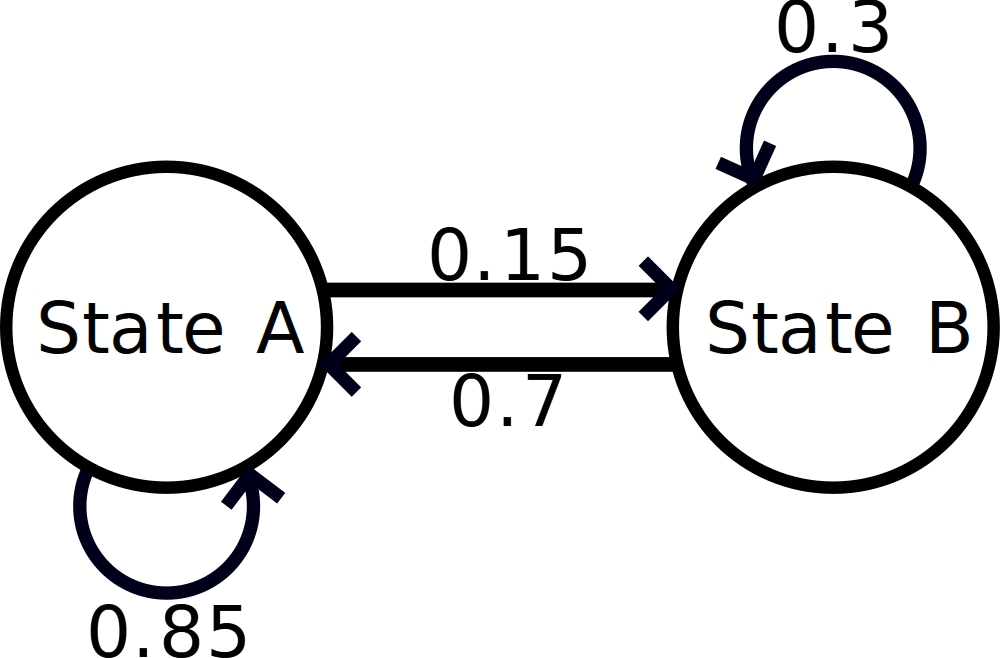
\includegraphics[width=0.33\textwidth]{images/markov-chain.png}
    \caption[Diagram: Markov Chain]{A simple markov chain displayed as a graph. The states are represented as vertices. All possible transitions between states are denoted as edges. The edge weights define the probability of the transition relative to all other outgoing edges of a node.}
    \label{fig:markovchain}
\end{figure}

\subsubsection{Data Structure and Algorithm}
In order to get the best results, the recommender system should save all combinations of items that have previously been searched for together and then recommend
the next one based on this exact starting point. On the downside, this would result in a lot of different origin states that contain very few possible future states due to being overly specific to a single search. The stored data can only be used if the exact same combination of skills is entered again.\\
Another way to implement such a recommendation engine would be to only inspect the last entered search item and ignoring all other ones. Given $n$ known skill items, all probabilities for the future state could be saved in one single $n \times n$ matrix saving only $n^2$ values.
This solution would disregard the whole context of the search item.\\
As a tradeoff, the system will generate predictions for each skill in the search query independently and aggregate these predictions afterward. For each skill, a list of possible recommendations paired with the total count of searches for both will be stored. The recommendation lists of all skills combined represent the transition matrix. Instead of transition probabilities, the total number of searches is saved in order to simplify the aggreation of multiple suggestions.\\
The recommender system will concatenate the suggestion lists of all items in the current search query and add up the counts of skills appearing in multiple suggestion lists. Then, all elements of the combined list that are part of the search query will be removed, the result is a list of suggestions for the whole search query.\\

\newpage
\subsection{Pseudo-Code}
\begin{figure}[h]
\begin{lstlisting}[language=Java]
var knownSkills = [
  {
    name: "java",
    similar: [
      {
        name: "php",
        count: 3
      }, {
        name: "ruby",
        count: 2
      }
    ]
  }, {
    name: "php",
    similar: [
      {
        name: "java",
        count: 5
      }, {
        name: "ruby",
        count: 2
      }
    ]
    name: "ruby",
    similar: [
      {
        name: "java",
        count: 0
      }, {
        name: "php",
        count: 5
      }
    ]
  }
]
\end{lstlisting}
\caption[Data Structure: Known Skill]{Pseudo-Implementation of the known skills' data structure}
\end{figure}

\newpage

\begin{figure}
\begin{lstlisting}[language=Java]
function suggest(searched) {
  var accumulated = {};

  for (s in searched) {
    for (t in knownSkills.getByName(t).getSkillsSearchedWith()) {
      if (accumulated.getByName(t) exists) {
        accumulated.getByName(t).count += t.count
      } else {
        accumulated.getByName(t) = t.clone()
      }
    }
  }

  for (t in accumulated) {
    if (searched contains t) {
      remove t from accumulated
    }
  }

  return accumulated.getHighestCount();
}

\end{lstlisting}
\caption[Pseudocode: Skill Suggestion Algorithm]{Pseudo-Implementation of the suggestion of a known skill based on a set of already searched items.}
\end{figure}

\subsection{Example}
Let there be the following transition matrix:

\begin{center}
\begin{tabular}{c | c |c | c | c}
		  & Java & PHP & CSS & COBOL\\
	\hline
	Java  &  -   &  7  &  3  &   1  \\
	\hline
	PHP   &  7   &  -  &  9  &   5  \\
	\hline
	CSS   &  3   &  9  &  -  &   8  \\
	\hline
	COBOL &  1   &  5  &  8  &   -  \\
\end{tabular}
\end{center}

Using the given transition matrix and the search query ``Java, PHP'', the algorithm works like this:
\begin{enumerate}
	\item Retrieve suggestion lists for each search item\\
		$\Rightarrow$ PHP (7), CSS (3), COBOL (1), Java (7), CSS (9), COBOL (5)
	\item Aggregate lists (combine counts)\\
		$\Rightarrow$ PHP (7), Java (7), CSS (12), COBOL (6)
	\item Remove suggestions that are part of the search query\\
		$\Rightarrow$ CSS (12), COBOL (6)
	\item Suggest item with the highest total count\\
		$\Rightarrow$ CSS
\end{enumerate}

\begin{figure}[!htp]
    \centering
    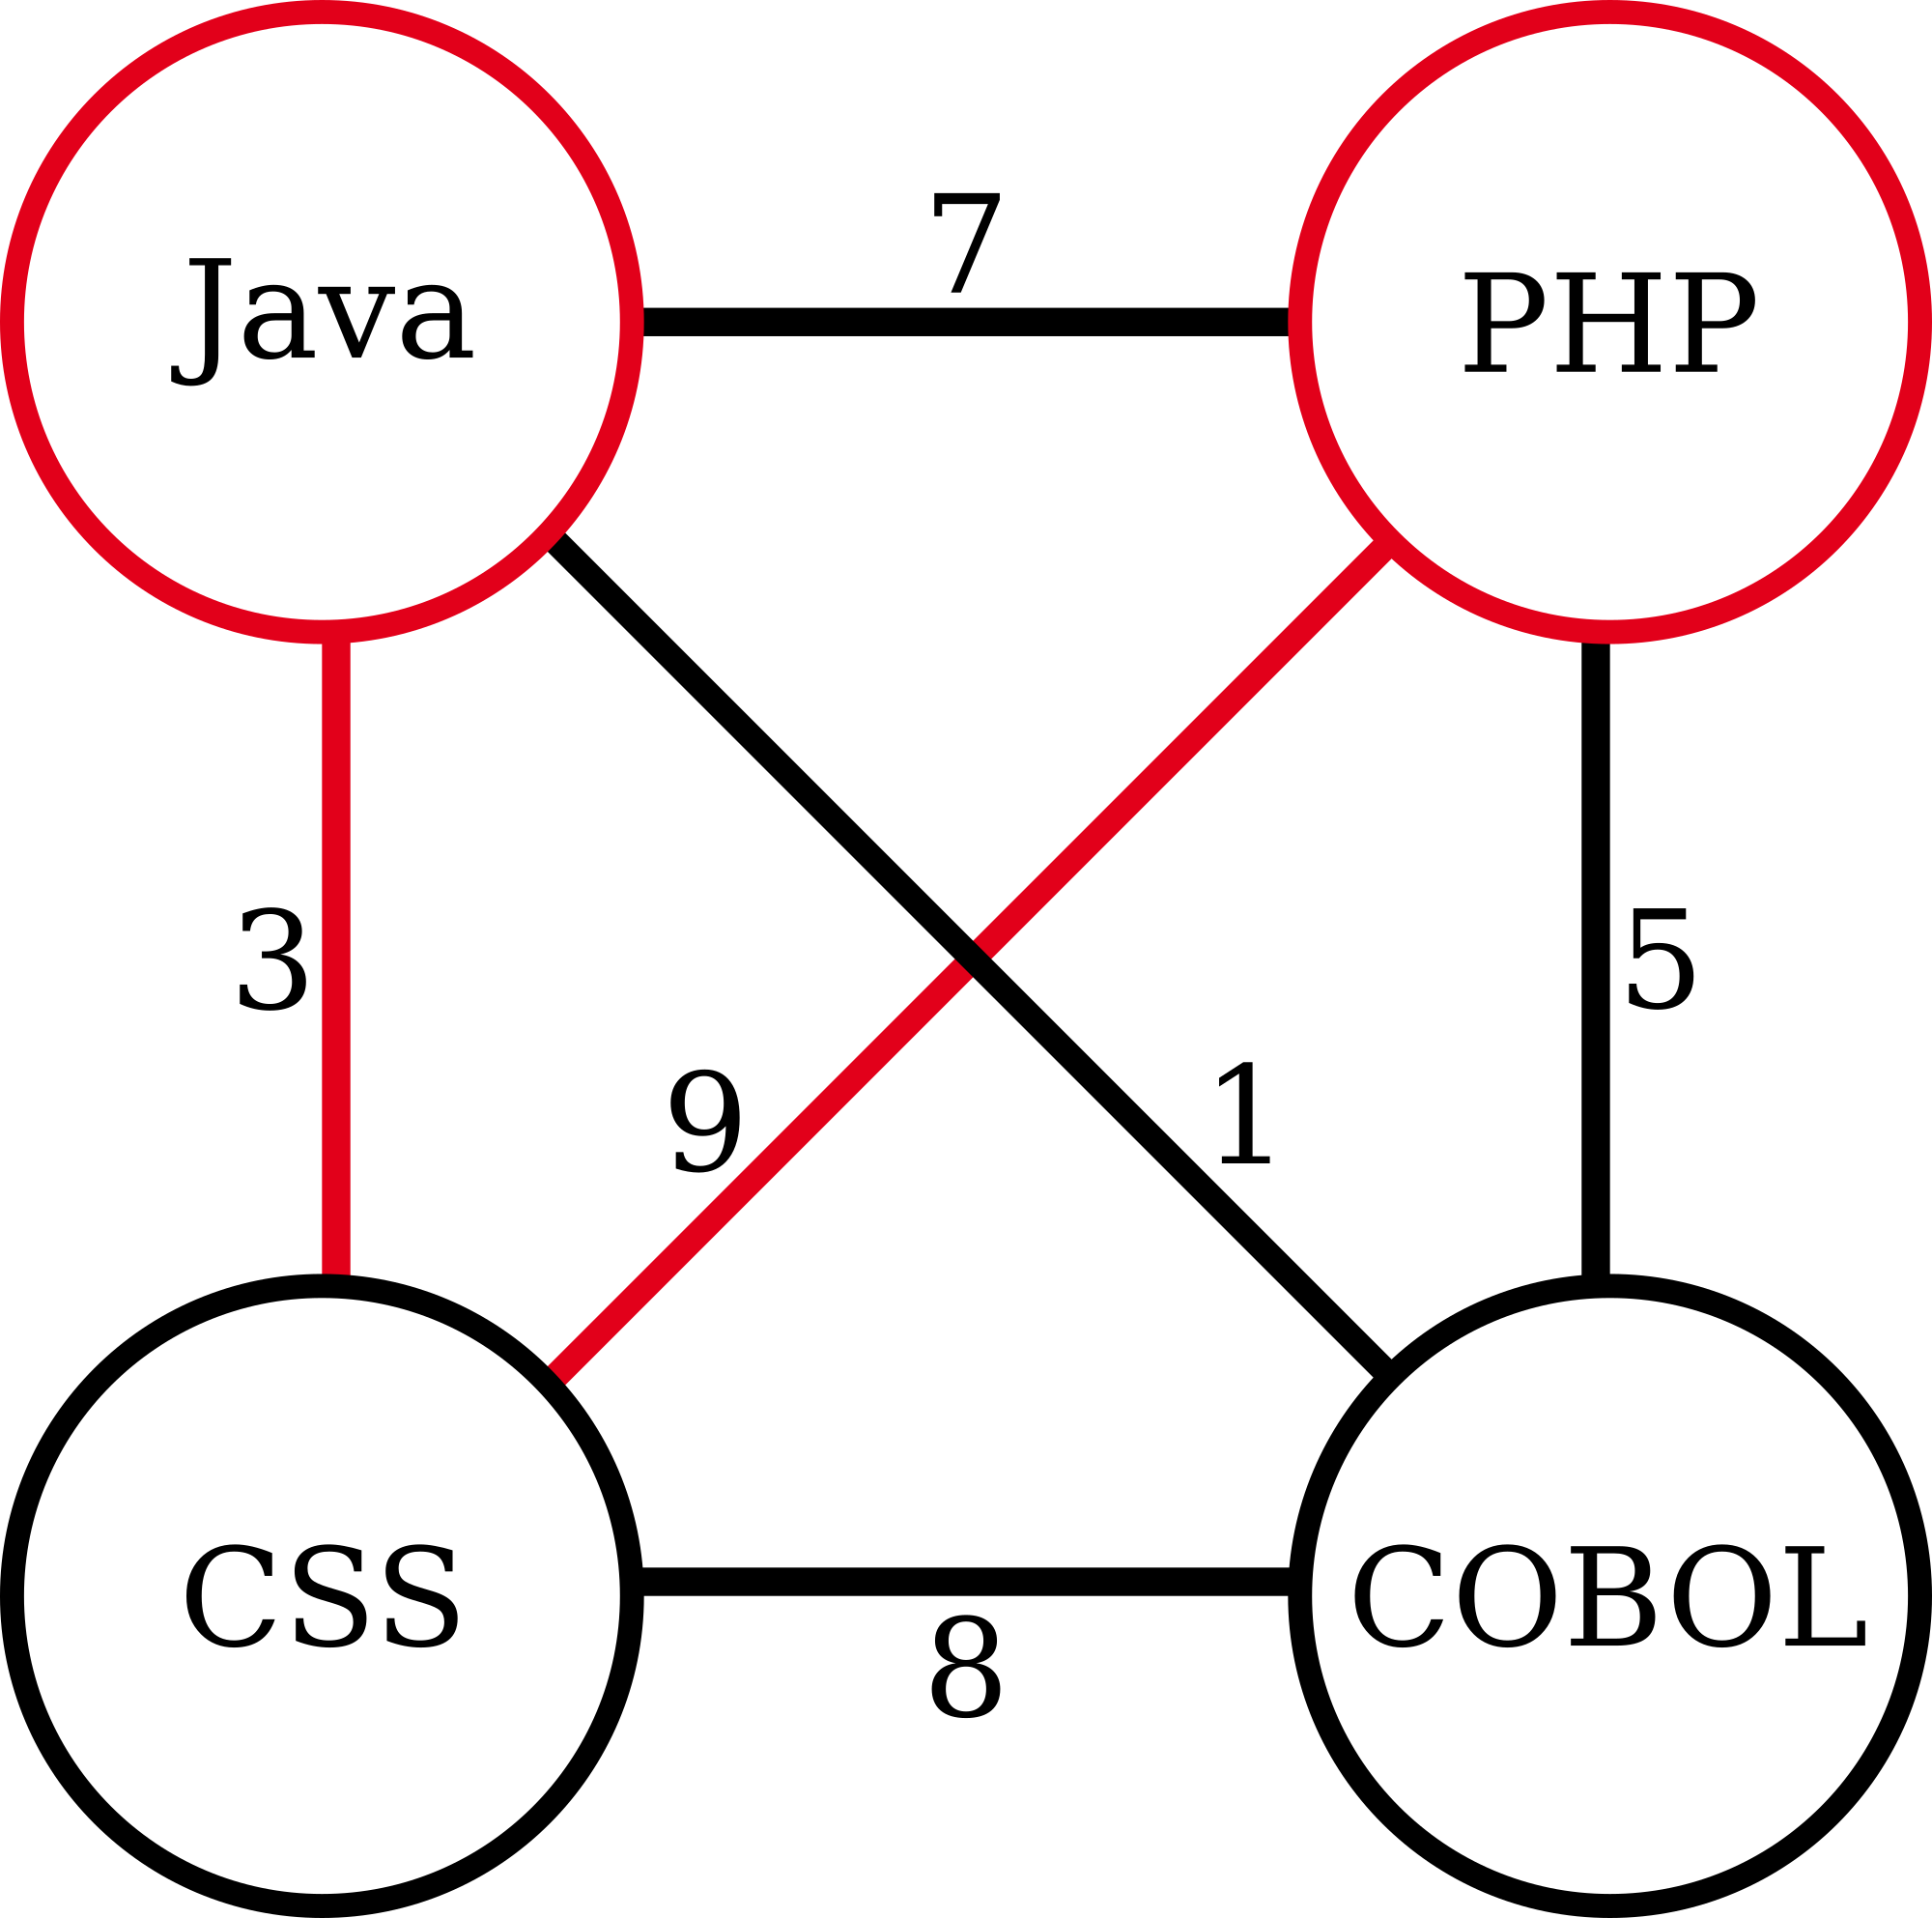
\includegraphics[width=0.33\textwidth]{images/markov_impl.png}
    \caption[Diagram: Search Suggestion Markov Model]{Markov Model used in the example. The two origin states and the transitions that form the end result are highlighted red.}
    \label{fig:wireframe}
\end{figure}

\section{Visual Concept \& Wireframes}
The application should be as simple as possible and usable for everyone in order to provide an efficient and fast tool. Thus, it will be designed as a single page application based around a search function that provides a way to input the skills needed and returns all persons offering said skills. After entering a search, the user can select any of the found colleagues and view their personal profile showing extended information like contact details, more skills the user did not search for, and the employee's location. This profile will also include links to directly contact the inspected person via e-mail or \textit{Google Hangouts}\footnote{https://hangouts.google.com}. Unlike the considered commercial solutions (see \ref{commercial}), this tool will not include features like creating statistics, assessments, applicant management, or any dashboard other than the basic search view.
Furthermore, there will not be any role model to differentiate between ``regular'' employees and managers since this application is meant to be a tool enhancing collaboration, not supervision. More information about the concept behind the visual design and the frontend's implementation is provided by Strecker \cite{strecker}.
\newpage
\begin{figure}[hp]
    \centering
    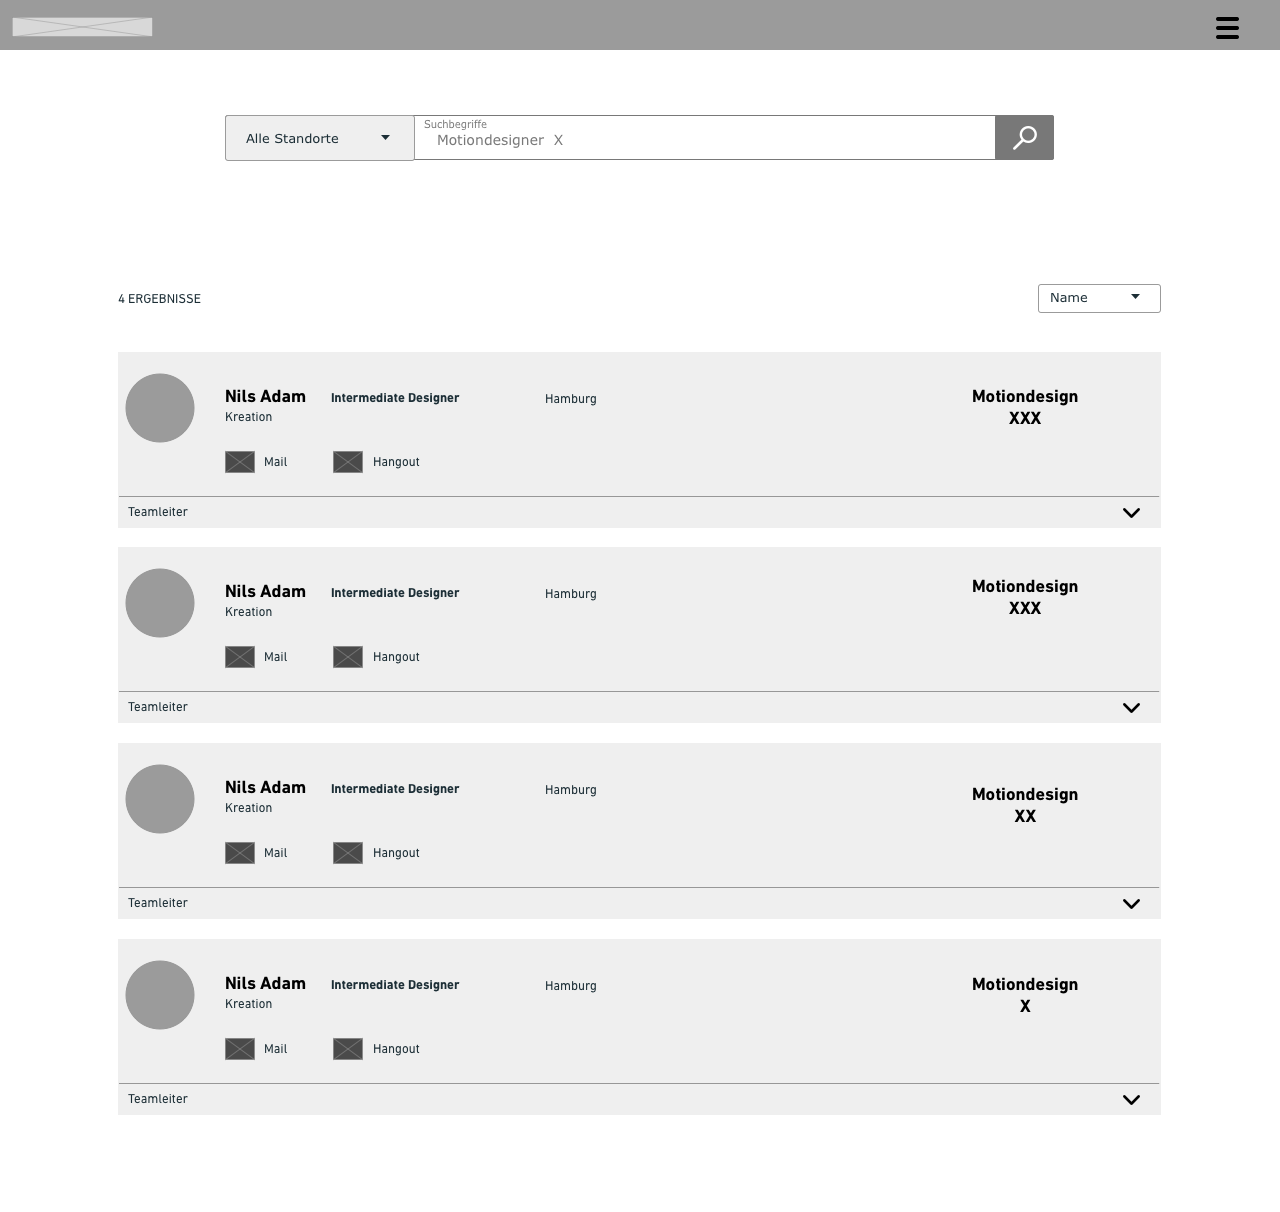
\includegraphics[width=\textwidth]{images/wireframe.png}
    \caption[Illustration: Search Result Page (Wireframe)]{Wireframe of the search result view}
    \label{fig:wireframe}
\end{figure}
\newpage
\begin{figure}[hp]
    \centering
    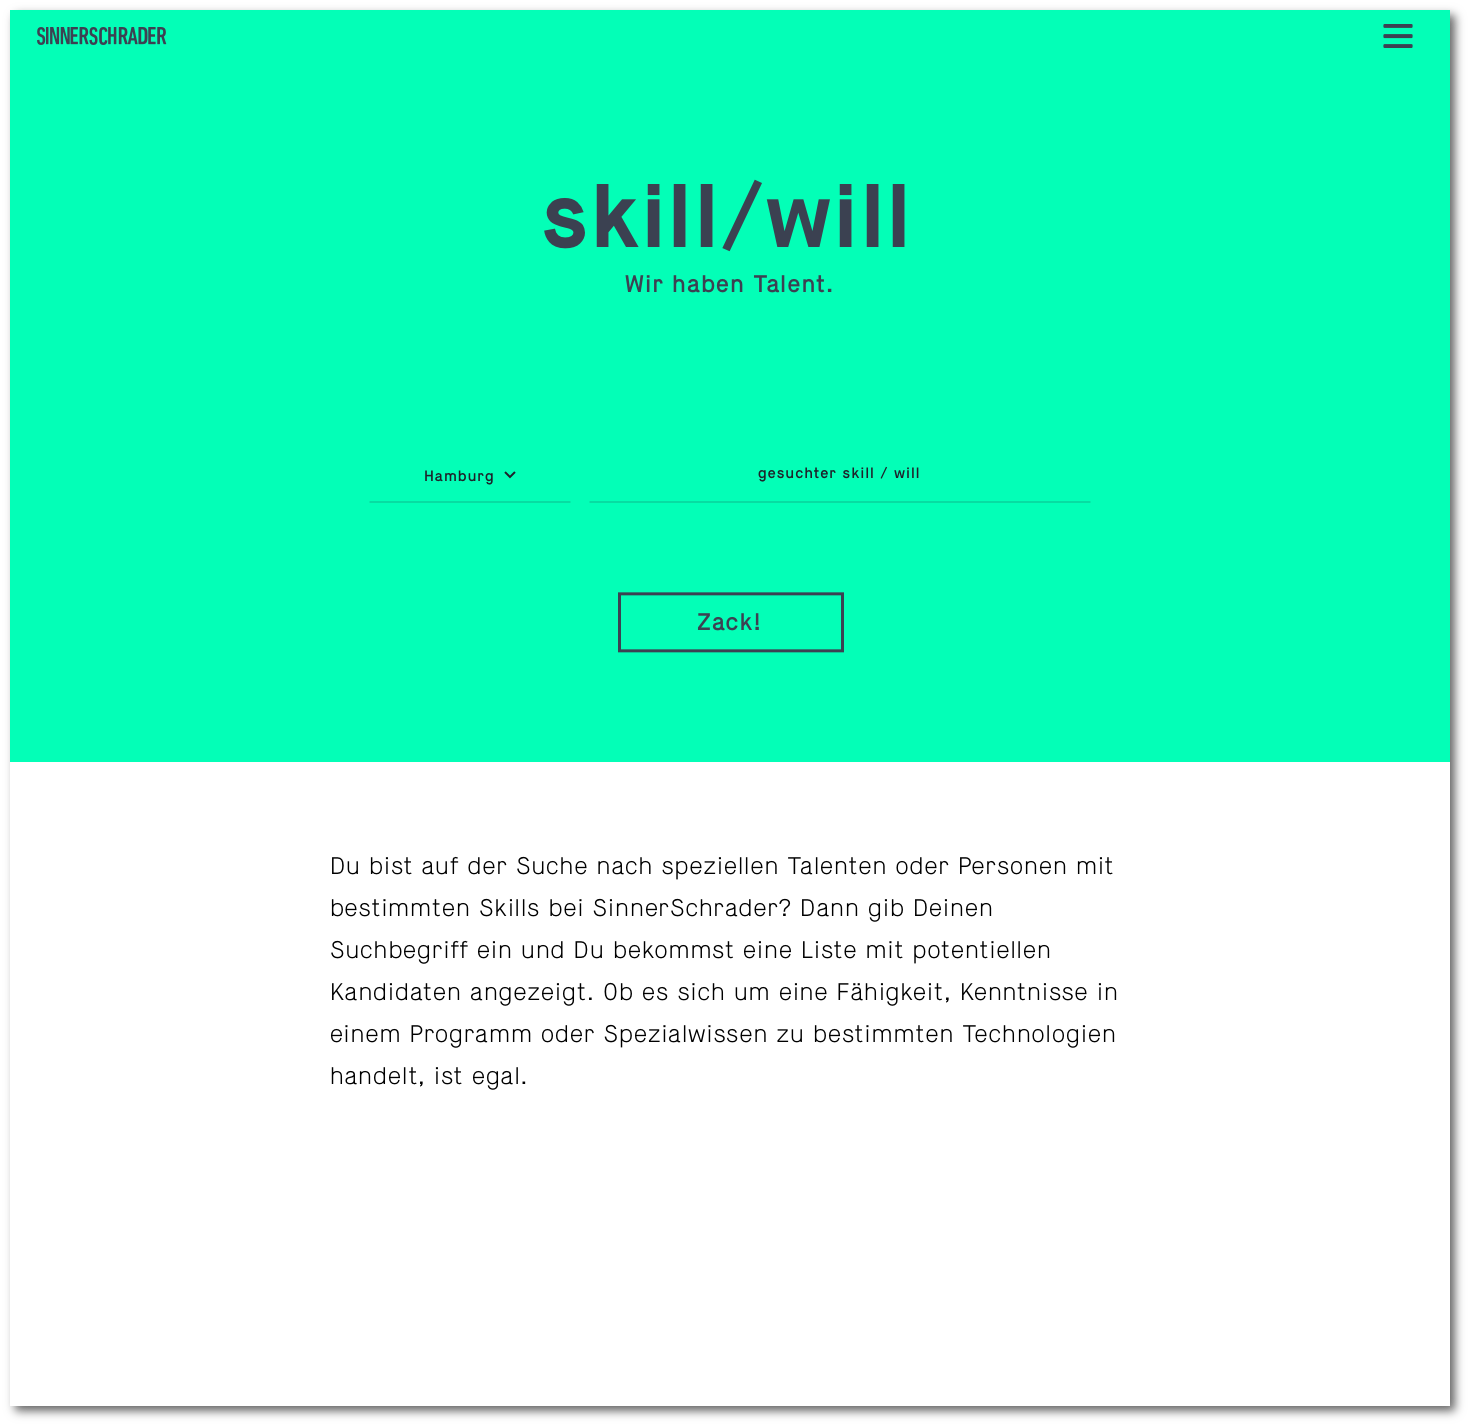
\includegraphics[width=\textwidth]{images/design_home.png}
    \caption[Illustration: Search Page (Concept)]{An early prototypical design for the search view}
    \label{fig:design_home}
\end{figure}
\newpage

\section{Legal Concerns}
Nearly all of data fall into the category of personal data (\textit{Personenbezogene Daten}), which is defined as ``any information concerning the personal or material circumstances of an identified or identifiable individual (the data subject)'' (BDSG, 3(1)). The personal data will be collected (BDSG, 3(3)), processed (BDSG, 3(4)) and transferred (BDSG, 3(3)) to other employees of SinnerSchrader.
Generally, this does not violate any law, since the ``collection, storage, modification or transfer of personal data or their use as a means of fulfilling one’s own business purposes shall be admissible'' (BDSG, 28(1)), but some restrictions apply: the data subjects have to be informed about the processing of their personal data, they must be able to deny their consent (BDSG, Section 4a), and the personal data shall not be made public.
To ensure the latter, the application must not be accessible to persons that do not work for or on behalf of SinnerSchrader. Technically, this will be arranged by making the application attainable from SinnerSchrader's internal network only, which can exclusively be used by employees and authorized persons.

\chapter{Implementation}
\section{Application Structure}
The application consists of two main components: the frontend that presents the user with a graphical interface and the backend that provides data and actions on it to the frontend.
The user's browser connects to a web server that acts as a reverse proxy and not only provides static resources like HTML and CSS files which resemble the frontend, but also acts as an SSL endpoint.
Requests for dynamic data and actions that are handled via the REST API provided by the backend are passed on to it, its response will then be directed through the reverse proxy to the client.
To store and read data, the backend connects to a MongoDB Database. User details are synced from the existing LDAP server which acts a central repository for personal information of all employees.
\begin{figure}[h]
    \centering
    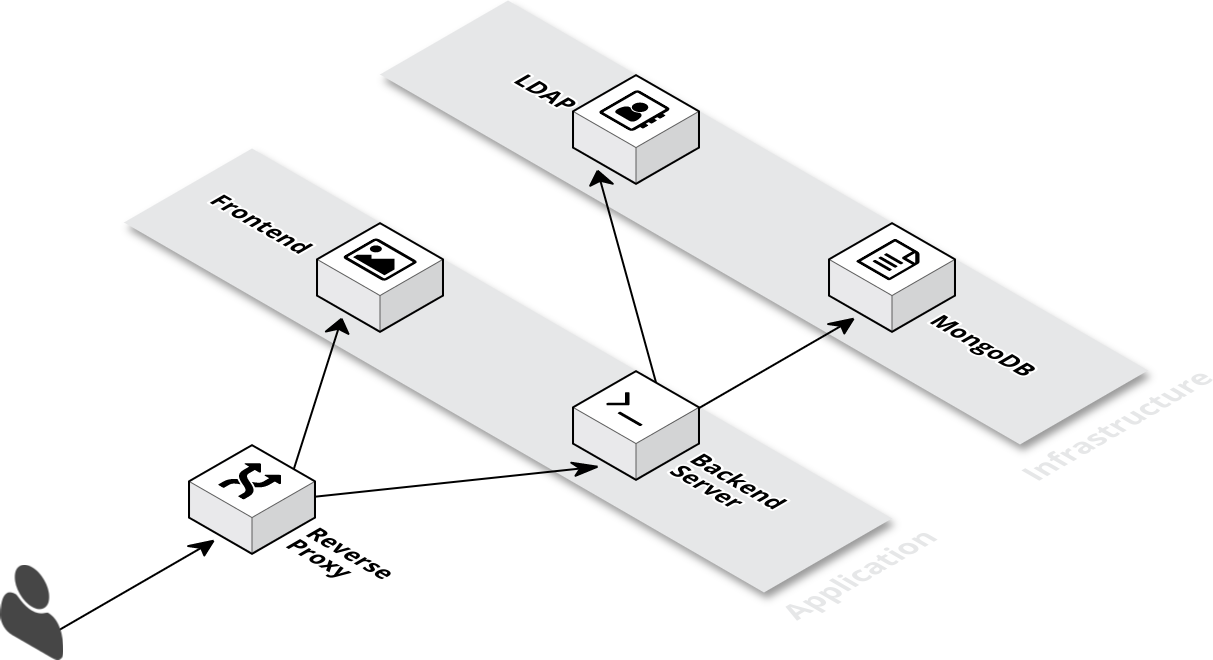
\includegraphics[width=\textwidth]{images/system_architecture.png}
    \caption[System Architecture]{The system's architecture. Created with \textit{https://cloudcraft.co}.}
    \label{fig:markovchain}
\end{figure}

\newpage
\section{MongoDB}
MongoDB\footnote{https://www.mongodb.com} is a popular non-relational NoSQL database that aims to be fast and easy to use \cite[p. 10]{MongoGuide}. To increase performance, like many NoSQL databases, it does not provide ACID\footnote{Atomicity, Consistency, Isolation, Durability} transactions which are a well-known feature of relational database management systems (RDBMS). This, however, simplifies horizontal scaling since new machines can easily be inserted into an existing cluster of database servers without the need to be in sync \cite[p. 3]{MongoGuide}.

\subsection{BSON}
\label{BSON}
In contrast to relational databases that store all data in tables, MongoDB uses a document-orient data structure saving every element in the Binary JSON\footnote{Javascript Object Notation} (BSON) format. This approach allows complex data to be stored as one object rather than having to dissect its elements and storing them in separate tables. As a consequence, retrieving an object from the database is much more efficient than it would be using an RDBMS, as the latter needs to join the tables storing the object's nested sub-objects and compose the requested element whereas MongoDB has it stored in the exact same form it is requested \cite[p. 10]{MongoGuide}.

\subsection{Data Structure}
The application stores three different object classes in the database: skills that are known to the system, persons with their individual contact data and skills, and sessions used to authenticate users that wish to modify their profiles. In order to instantiate the elements as java objects, Spring Data\footnote{http://projects.spring.io/spring-data/}, the framework used for database access, also stores the class name the object needs to be mapped to as a field inside of it. Furthermore, every item has the field \textit{version} which holds a version number used to resolve writing conflicts that may occur when multiple threads access the same object simultaneously.

\newpage
\subsubsection{Known Skills}
Skills known to the system consist of a unique name and a list of suggestions that themselves are expressed by a name and a total count of searches of the respective suggestion together with the skill.
\begin{figure}[h]
\begin{lstlisting}[language=Java]
{
  "_id" : "Java",
  "_class" : "[...].skills.KnownSkill",
  "suggestions" : [
    {
      "name" : "AEM",
      "count" : 1
    }, {
      "name" : "jquery",
      "count" : 1
    }
  ],
  "version" : NumberLong(3)
}
\end{lstlisting}
\caption[Skill (DB Data Structure)]{Data structure of a skill stored in the database}
\end{figure}

\subsubsection{Sessions}
Sessions are used to authenticate users that wish to modify their personal profile. The client has to authenticate the user with their credentials; if this is successful, a new session holding a unique id, the point of time it will expire, and the id of the authenticated user, will be created and stored in the database.

\begin{figure}[h]
\begin{lstlisting}[language=Java]
{
	"_id" : "87163f310f124830bac677fe31484262",
	"_class" : "com.sinnerschrader.skillwill.session.Session",
	"username" : "foobar",
	"expireDate" : ISODate("2017-01-09T08:36:40.128Z"),
	"version" : NumberLong(1)
}
\end{lstlisting}
\caption[Session (DB Data Structure)]{Data structure of a session stored in the DB}
\end{figure}
\newpage

\subsubsection{Persons}
\label{db:person}
The documents that represent persons contain the respective person's id\footnote{Each employee gets assigned an internal id (\textit{Benutzerkürzel}) that is globally used to uniquely identify a person.}, their personal data like first and last name, telephone number, e-mail address, office location, job title\footnote{The job title data is not maintained consistently in the LDAP, so that, unfortunately, it is not suitable to be used in the person search.}, and a list of the person's skills. Each of those skills consists of a name, a level of skill and a level of will.
\begin{figure}[h]
\begin{lstlisting}[language=Java]
{
  "_id" : "foobar",
  "_class" : "com.sinnerschrader.skillwill.domain.person.Person",
  "skills" : [
    {
      "_id" : ".NET",
      "skillLevel" : 1,
      "willLevel" : 2
    },{
      "_id" : "Scrum",
      "skillLevel" : 3,
      "willLevel" : 1
    }
  ],
  "version" : NumberLong(1),
  "ldapDetails" : {
    "firstName" : "Fooberius",
    "lastName" : "Bartels",
    "mail" : "foobar@mail.org",
    "phone" : "+49 12 345678 901",
    "location" : "Hamburg",
    "title" : "Development"
  }
}
\end{lstlisting}
\caption[Person (DB Data Structure)]{Data structure of a person stored in the DB}
\end{figure}

\newpage



\subsection{Queries}
As shown in \ref{BSON}, the document based data structure of MongoDB allows the database to efficiently perform complex requests. Furthermore, it provides simple and straightforward search queries to retrieve objects based on their attributes. For example, getting all users who offer the skill \textit{Ruby} from the collection \textit{person} can be done with this straightforward query:
\begin{figure}[h]
\begin{lstlisting}[language=Java]
db.person.find({ "skills._id" : "Ruby" })
\end{lstlisting}
\caption[Example Database Query]{MongoDB query to retrieve all users with the skill \textit{Ruby}}
\end{figure}

\section{LDAP}
SinnerSchrader runs an LDAP server which acts as a centralized source of personal information of all employees. The application connects to this server in order to retrieve contact information to display in users' profiles. In comparison with having the users to enter their data manually, this method has the benefit that the users' data will be kept in sync across all internal services, and that it reduces the effort a user has to spend to create their profile.

\section{Reverse Proxy}
Between the client and the backend, an intermediary web server that acts as a reverse proxy is switched in. Its main purpose is the distinguishing between requests for static files, like HTML and CSS content that will be directly delivered by said server, and API calls that are redirected to the backend. This increases the system's security by protecting the backend server's identity and presenting an additional defense layer \cite{NGINX}. Furthermore, this server can handle SSL encryption between the application and the client, and, if multiple backend servers are needed, balance the workload between them while presenting one uniform service to the outside.

\section{API}
To exchange data between the backend and the frontend, a \textit{Representational State Transfer} (REST) API is provided by the backend. Its endpoints are called by the fronted code to either request data or to command the backend to perform modifying operations on it.
The used HTTP method is the main indicator of the action to perform: GET is used to retrieve data, POST to insert new elements, PUT to modify existing ones and DELETE to remove them. The URLs of the individual action express the entity on which the action will be performed. All API endpoints are listed in table \ref{swaggertable}.

\begin{table}[p]
\centering
\rotatebox{-90}{
  \begin{tabular}{l|l|l|l|l}
  URL & HTTP Method & Non-URL Parameters & Return Status & Comment\\
  \hline
  /login               & POST   & username, password                          & 200, 401, 500           & Try to login a user;\\ & & & & returns session key\\ \hline
  /logout              & POST   & session                                     & 200, 401, 500           & Logout a session\\ \hline
  /skills              & GET    & search                                      & 200, 500                & Search for autocompletion;\\ & & & & returns all skills if search is empty\\ \hline
  /skills              & POST   & name                                        & 200, 400, 401, 500      & Add new skill with\\ & & & & the given name\\ \hline
  /skills/next         & GET    & search                                      & 200, 400, 500           & Suggest a skill based on\\ & & & & the comma separated list of\\ & & & &   skills (parameter: search)\\ \hline
  /skills/\{skill\}      & DELETE &                                             & 200, 400, 401, 404, 500 & Remove the skill\\ & & & &  with the given name\\ \hline
  /skills/\{skill\}      & PUT    & name                                        & 200, 400, 401, 404, 500 & Rename the skill\\
  /users               & GET    & skills, location                            & 200, 400, 500           & Get all users\\ & & & &  matching the searched\\ & & & & skills in the given location\\ & & & & (parameters may be empty)\\ \hline
  /users/\{user\}        & GET    &                                             & 200, 404, 500           & Return the specified user\\ \hline
  /users/\{user\}/skills & POST   & session, skill, skill\_level, will\_level & 200, 400, 401, 404, 500 & Create new skill/modifiy existing\\ & & & & personal skill\\ \hline
  /users/\{user\}/skills & DELETE & session, skill                              & 200, 400, 401, 404, 501 & Remove the skill\\ & & & & from the users profile\\
  \end{tabular}
  }
\caption[API Endpoints]{All API endpoints provided by the backend}
\label{swaggertable}
\end{table}
\newpage

\subsection{API Responses}
The API returns data in the JSON format, which is one of the two de-facto standards for data exchange on the web\footnote{The other one is \textit{XML} used by the \textit{Simple Object Access Protocol}} because it is part of the Javascript (JS) language \cite[p. 37]{json}. Approximately 94\% of all websites use JS \cite{jsmarket}; since JSON directly represents JS objects and is both easy to parse and human-readable, it became the leading data format for web applications.
For every HTTP request, the backend will return a JSON response, notwithstanding the request may not demand data to be returned. In this case, the response will contain status information about the success of the requested action.

\begin{figure}[h]
\begin{lstlisting}[language=Java]
{
	"id" : "foobar",
	"firstName" : "Fooberius",
	"lastName" : "Bartels",
	"mail" : "foobar@mail.org",
	"phone" : "+49 12 345678 901",
	"location" : "Hamburg",
	"title" : "Development",
	"skills" : [
		{
			"name" : ".NET",
			"skillLevel" : 1,
			"willLevel" : 2
		}, {
			"name" : "Scrum",
			"skillLevel" : 3,
			"willLevel" : 1
		}
	]
}
\end{lstlisting}
\caption[Person API Response]{Example JSON response by the API for the request \textit{/users/foobar}. For comparison, the corresponding database entry is shown in \ref{db:person}.}
\end{figure}


\begin{figure}[h]
\begin{lstlisting}[language=Java]
{
	"message" : "logout successful"
}
\end{lstlisting}
\caption[Status API Response]{Example JSON response for a request that does not demand any data.}
\end{figure}


\section{Backend}
\label{impl:be}
The backend component ist implemented in Java 8\footnote{https://go.java/} using the Spring Boot framework\footnote{https://projects.spring.io/spring-boot/}. Maven\footnote{https://maven.apache.org/what-is-maven.html} is employed to manage the build process and run unit and integration tests.

\section{Architecture}
The software architecture consists of three main categories of classes: services handling data manipulation and filtering that hold the business logic, repository objects that wrap the database operations into easy to use handlers, and domain specific data types. Additionally, numerous helper classes like custom exception types, comparators, and general utilities are implemented.
\begin{figure}[!h]
    \centering
    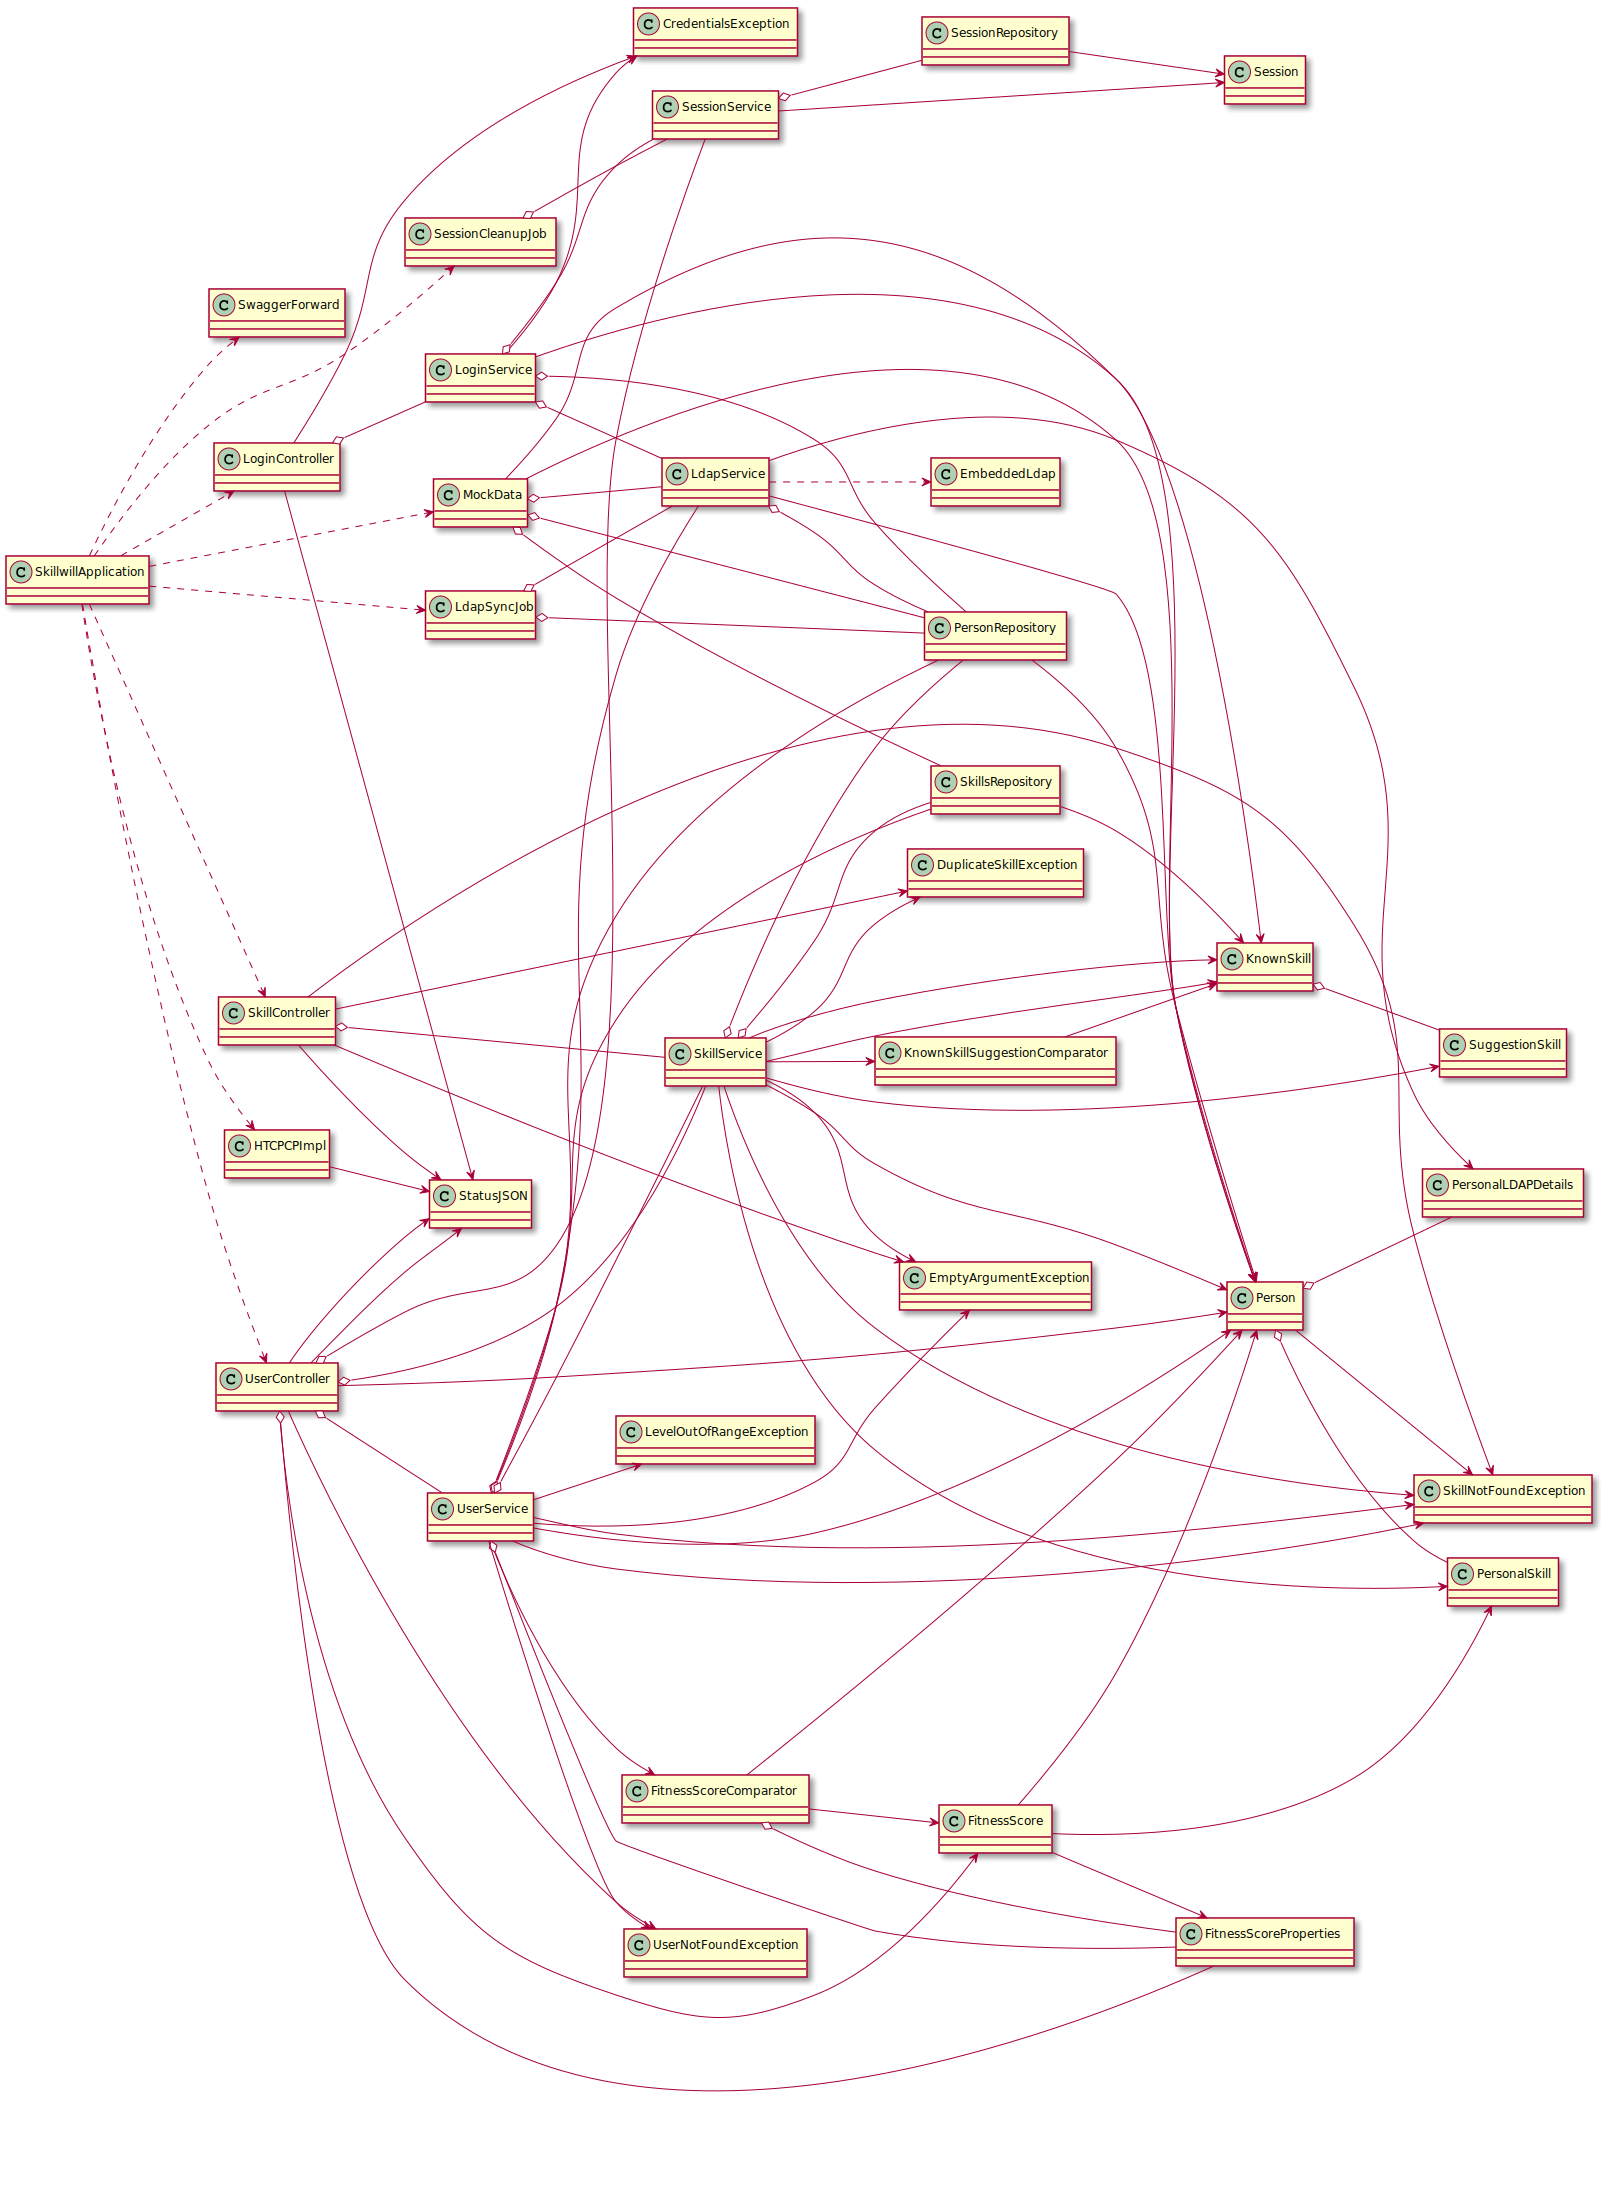
\includegraphics[height=0.55\textheight]{images/uml.png}
    \caption[Backend Class Diagramm]{UML class diagram of the backend to illustrate its dimensions.}
    \label{fig:markovchain}
\end{figure}
\newpage

\subsection{Spring Boot}
\textit{Spring Boot} is a highly sophisticated web framework that provides numerous features to create web applications including, but not limited to, annotations to expose java methods as HTTP request endpoints, an embedded webserver to run the application on, a modular design to extend its features, and dependency injection. It is used because its credo to provide default configurations where possible and thus reduce the need to write infrastructure code simplifies the applications' structure \cite[p. 6]{SpringGuide}.
For example, a controller that returns a static response can be created using two annotations:
\textit{@Controller} to make Spring Boot identify the class as a resource that will listen to HTTP calls, and \textit{@Request} to specify the URL and HTTP method to use. Unlike most other web frameworks, spring boot does not require any more configuration or dispatching classes.

\begin{figure}[h]
\begin{lstlisting}[language=Java]
@Controller
public class HTCPCPImpl {

	@RequestMapping(path = "/coffee", method = RequestMethod.GET)
	public ResponseEntity<String> coffee() {
		StatusJSON json = new StatusJSON("I'm a teapot \u2615");
		return new ResponseEntity<String>(
      json.toString(),
      HttpStatus.I_AM_A_TEAPOT
    );
	}

}
\end{lstlisting}
\caption[Example Controller]{Example controller using Spring Boot}
\end{figure}

\newpage
\subsection{Spring Data Repositories}
\textit{Spring Data}\footnote{http://projects.spring.io/spring-data/} is a module for Spring Boot that streamlines the way elements can be accessed from a database.
The components mainly used in this application are CRUD\footnote{Create, Read, Update, Delete} repository objects that enclose the database connections and serve
simple java methods as an interface. To create such a repository, a java interface defining the stored data type and custom database queries has to be constructed.
No actual implementation of the interface has to be created since it will be generated automatically by Spring Data.
The parameters needed to connect to the database have to be configured in any source of properties known to Spring Boot, e.g. in \textit{src/main/resources/application.properties}.

\begin{figure}[h]
\begin{lstlisting}[language=Java]
public interface PersonRepository
		extends MongoRepository<Person, String> {

	Person findById(String id);

	@Query("{ skills._id : ?0 }")
	List<Person> findBySkill(String skillName);

}
\end{lstlisting}
\caption[Example Repository Interface]{Example for a repository interface managing person objects stored in the database.}
\end{figure}

\begin{figure}[h]
\begin{lstlisting}[language=Java]
spring.data.mongodb.host=127.0.0.1
spring.data.mongodb.port=27017
spring.datasource.driverClassName=com.mongodb.Mongo
\end{lstlisting}
\caption[Spring Data Config]{All configuration parameters needed to run Spring Data}
\end{figure}

\subsection{LDAP Connection}
To connect to the LDAP server, the \textit{unboundid} library is used in the class \textit{LdapService}, It provides methods to open a TCP connection to the server, make requests, and parse the server's response. The connection to the LDAP server will be kept alive and is reused for all operations, so that the effort to open a new connection is eliminated.

\begin{figure}[H]
\begin{lstlisting}[language=Java]
@Service
@Scope("singleton")
@EnableRetry
public class LdapService {

	private static Logger logger =
    LoggerFactory.getLogger(LdapService.class);

	// [fields not used in this example]

	private static LDAPConnection ldapConnection;

	@Autowired
	private PersonRepository personRepo;

	// [methods for user sync and connection handling]

	public boolean canAuthenticate(String username,
			String password) {
		try {
			BindRequest bindRequest = new SimpleBindRequest(
				"uid=" + username + "," + ldapBaseDN, password);
			BindResult bindResult =
				ldapConnection.bind(bindRequest);
			if (bindResult.getResultCode()
					.equals(ResultCode.SUCCESS)) {
				return true;
			}
			return false;
		} catch (LDAPBindException e) {
			return false;
		} catch (LDAPException e) {
			logger.error("Failed to authenticate: LDAP error");
		}
		return false;
	}

}
\end{lstlisting}
\caption[LDAP User Authentication (Code)]{LDAP user authentiction using the unboundid library. Note: parts of the code have been removed for this example.}
\end{figure}


\subsection{Swagger}
\textit{Swagger}\footnote{http://swagger.io/} is an open source framework for creating documentations of REST APIs.
Its annotation based java integration is heavily used to generate an interactive overview of the API endpoints provided by the
backend. This overview is automatically served by spring boot and contains a list of all URLs to make requests to, HTTP response codes to expect, the content type of the response and a built in form to make example requests. The main advantage of this approach is that the code and its documentation are located at the very same place and that parts of the documentation are automatically generated, so that both are maintained synchronously, thus avoiding the documentation differing from the implementation.
\begin{figure}[H]
    \centering
    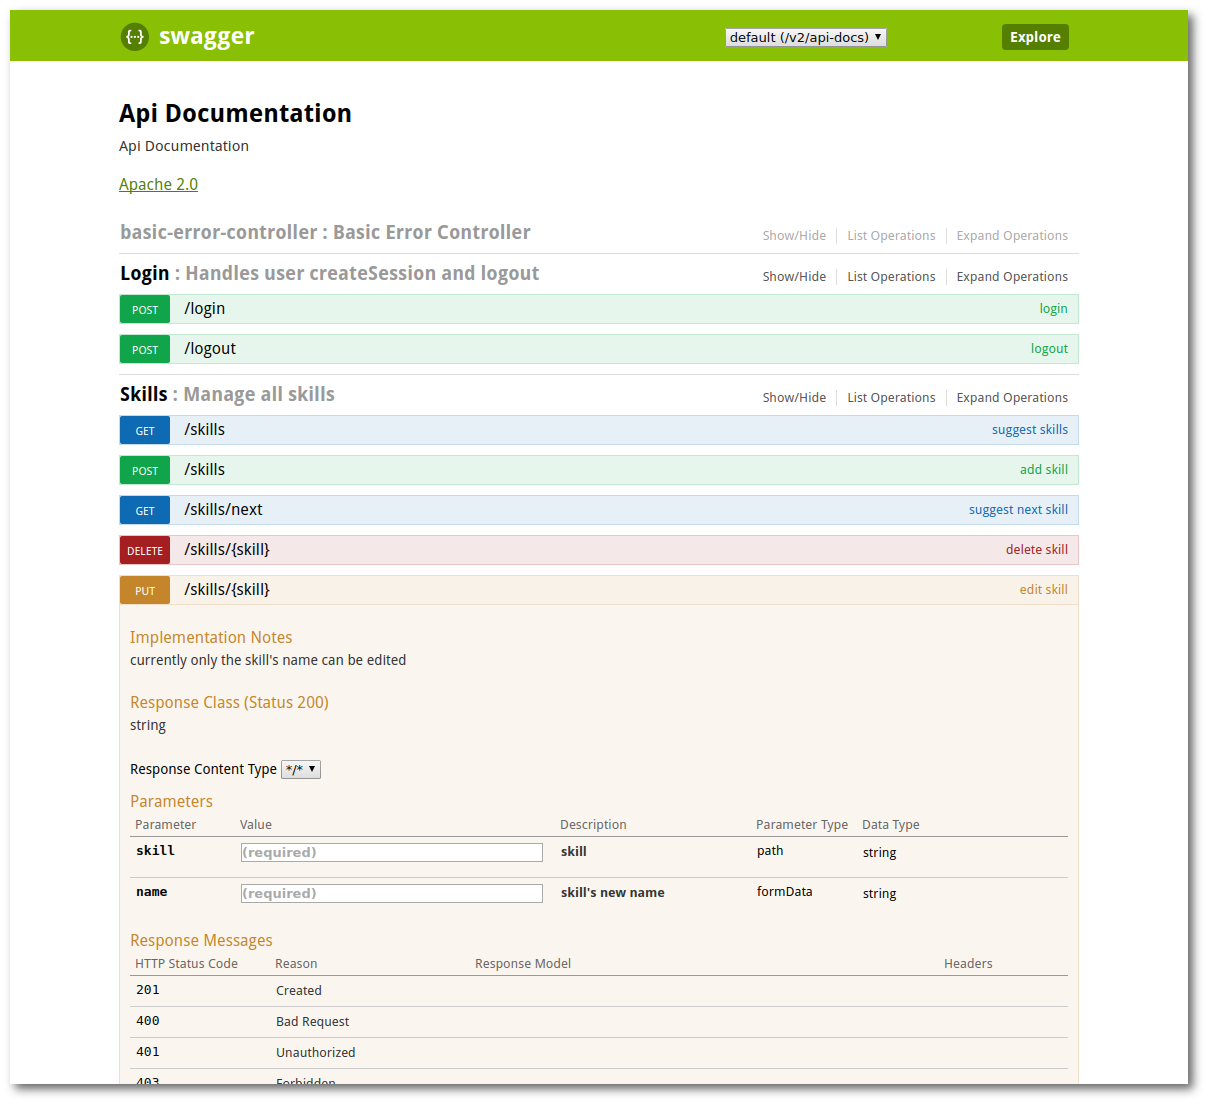
\includegraphics[width=\textwidth]{images/swagger_ui.png}
    \caption[Swagger Interactive Documentation]{Interactive API documentation generated by Swagger}
    \label{fig:markovchain}
\end{figure}

\subsection{Testing}
As a part of the build process, automatic tests are run using the \textit{JUnit}\footnote{http://junit.org} framework. Two types of tests are employed to ensure the proper working of the software: unit tests that validate isolated segments (java classes), and integration tests that simulate calls to the controllers and test the
interplay of the individual components.

\begin{figure}[h]
\begin{lstlisting}[language=Java]
@RunWith(SpringJUnit4ClassRunner.class)
@SpringBootTest
public class KnownSkillSuggestionComparatorTest {

	@Test
	public void testNoneStarts() {
		KnownSkill a = new KnownSkill("Wurstwasser");
		KnownSkill b = new KnownSkill("foo");

		List<KnownSkill> toSort = new ArrayList<KnownSkill>();
		toSort.add(a);
		toSort.add(b);
		toSort.sort(new KnownSkillSuggestionComparator("42"));

		assertEquals(a, toSort.get(0));
		assertEquals(b, toSort.get(1));
	}

	@Test
	public void bothStart() {
		KnownSkill a = new KnownSkill("foobar");
		KnownSkill b = new KnownSkill("foowurst");

		List<KnownSkill> toSort = new ArrayList<KnownSkill>();
		toSort.add(a);
		toSort.add(b);
		toSort.sort(new KnownSkillSuggestionComparator("foo"));

		assertEquals(a, toSort.get(0));
		assertEquals(b, toSort.get(1));
	}

}
\end{lstlisting}
\caption[Example Unit Test]{Example unit test using JUnit}
\end{figure}


\subsubsection{Embedded Services}
During the integration test phase, external services like LDAP and a database have to be accessed in order to ensure the proper working of the interfaces connecting to them. Using the real services, however, is not an option as it cannot be assumed that the machine that runs the tests has a connection to them, and because the tests have to take control over the state of the services. To solve this, an LDAP server and a MongoDB are embedded into the application and will be used during testing.
The embedded database is the MongoDB implementation by \textit{flapdoodle}\footnote{https://github.com/flapdoodle-oss/de.flapdoodle.embed.mongo}, which has the advantage of being effortlessly deployed by importing it; all further configuration and setup happen automatically.
To embed an LDAP service, the \textit{unboundid} framework\footnote{https://www.ldap.com/unboundid-ldap-sdk-for-java} is used.

\section{License}
The software is licensed under the MIT license \cite{license} which is considered one of the most popular open source licenses, mainly because it grants a high level of freedom to modify and use the software under the sole condition that a copy of the original license is distributed algonside the software.

\begin{quote}
Copyright 2017 SinnerSchrader Deutschland GmbH

Permission is hereby granted, free of charge, to any person obtaining a copy of this software and associated documentation files (the "Software"), to deal in the Software without restriction, including without limitation the rights to use, copy, modify, merge, publish, distribute, sublicense, and/or sell copies of the Software, and to permit persons to whom the Software is furnished to do so, subject to the following conditions:

The above copyright notice and this permission notice shall be included in all copies or substantial portions of the Software.

THE SOFTWARE IS PROVIDED "AS IS", WITHOUT WARRANTY OF ANY KIND, EXPRESS OR IMPLIED, INCLUDING BUT NOT LIMITED TO THE WARRANTIES OF MERCHANTABILITY, FITNESS FOR A PARTICULAR PURPOSE AND NONINFRINGEMENT. IN NO EVENT SHALL THE AUTHORS OR COPYRIGHT HOLDERS BE LIABLE FOR ANY CLAIM, DAMAGES OR OTHER LIABILITY, WHETHER IN AN ACTION OF CONTRACT, TORT OR OTHERWISE, ARISING FROM, OUT OF OR IN CONNECTION WITH THE SOFTWARE OR THE USE OR OTHER DEALINGS IN THE SOFTWARE.
\end{quote}\cite{license}

%\include{kapitel2}
%\include{kapitel3}
%\include{kapitel4}
%\include{kapitel5}
%\include{kapitel6}
%\include{kapitel7}
% \cleardoublepage

% VERZEICHNISSE (Abbildungen, Tabellen)
% Literatur
% \nocite{wiki:wissarbeit}
\bibliographystyle{alphadin}
\bibliography{Bachelorarbeit}
\listoffigures
% \cleardoublepage

% ERKLÄRUNG
\addcontentsline{toc}{chapter}{Formalities (DE)}

\chapter*{Eidesstattliche Versicherung}
\markboth{Formalities (DE)}{Formalities (DE)}
Hiermit versichere ich an Eides statt, dass ich die vorliegende Arbeit im
Bachelorstudiengang Software-System-Entwicklung selbstständig verfasst und
keine anderen als die angegebenen Hilfsmittel – insbesondere keine im
Quellenverzeichnis nicht benannten Internet-Quellen – benutzt habe. Alle Stellen,
die wörtlich oder sinngemäß aus Veröffentlichungen entnommen wurden, sind als
solche kenntlich gemacht. Ich versichere weiterhin, dass ich die Arbeit vorher nicht
in einem anderen Prüfungsverfahren eingereicht habe und die eingereichte
schriftliche Fassung der auf dem elektronischen Speichermedium entspricht.

\vspace{2cm}

\noindent Hamburg, den \uline{~~~~~~~~~~~~~~~~~~~~}~~~~~Unterschrift: \uline{~~~~~~~~~~~~~~~~~~~~~~~~~~~~~~~~~~~~~~~~~~~~~~~~~~}


\chapter*{Einstellung in die Fachbereichsbibliothek}
\markboth{Formalities (DE)}{Formalities (DE)}
Ich bin mit einer Einstellung dieser Arbeit in den Bestand der Bibliothek des Fachbereiches Informatik an der Uni Hamburg einverstanden.

\vspace{2cm}

\noindent Hamburg, den \uline{~~~~~~~~~~~~~~~~~~~~}~~~~~Unterschrift: \uline{~~~~~~~~~~~~~~~~~~~~~~~~~~~~~~~~~~~~~~~~~~~~~~~~~~}


\end{document}
